\documentclass[12pt,a4paper]{report}

\usepackage[a4paper,margin=2.5cm]{geometry}
\usepackage[T1]{fontenc}
\usepackage[utf8]{inputenc}
\usepackage{lmodern}
\usepackage{microtype}
\usepackage{xcolor}
\usepackage{graphicx}
\usepackage{booktabs}
\usepackage{longtable}
\usepackage{tabularx}
\usepackage{array}
\usepackage{enumitem}
\usepackage{listings}
\usepackage{caption}
\usepackage{subcaption}
\usepackage{tikz}
\usetikzlibrary{arrows.meta,positioning,fit,shapes.geometric,shapes.misc,calc}
\usepackage[hidelinks]{hyperref}
\usepackage{fancyhdr}
\usepackage{titlesec}

\definecolor{ink}{HTML}{111111}
\definecolor{softink}{HTML}{444444}
\definecolor{linegray}{HTML}{D8D8D8}
\definecolor{papergray}{HTML}{F6F6F6}
\definecolor{codebg}{HTML}{F7F7F4}
\definecolor{codekw}{HTML}{1D4E89}
\definecolor{codestr}{HTML}{2E7D32}
\definecolor{codecomment}{HTML}{6A737D}
\definecolor{codered}{HTML}{8A1C1C}
\definecolor{accent}{HTML}{0F7B3F}

\hypersetup{
  pdftitle={A Lightweight Serverless Execution Platform},
  pdfauthor={Ilya},
  pdfsubject={Bachelor Project Prototype Documentation},
  pdfkeywords={serverless, orchestration, Docker, Redis Streams, Django, distributed systems}
}

\pagestyle{fancy}
\setlength{\headheight}{15pt}
\fancyhf{}
\fancyhead[L]{Lightweight Serverless Platform}
\fancyhead[R]{\thepage}
\renewcommand{\headrulewidth}{0.4pt}

\titleformat{\chapter}{\normalfont\huge\bfseries}{\thechapter}{1em}{}
\titleformat{\section}{\normalfont\Large\bfseries}{\thesection}{0.8em}{}
\titleformat{\subsection}{\normalfont\large\bfseries}{\thesubsection}{0.6em}{}

\lstdefinestyle{platformcode}{
  backgroundcolor=\color{codebg},
  basicstyle=\small\ttfamily,
  keywordstyle=\color{codekw}\bfseries,
  stringstyle=\color{codestr},
  commentstyle=\color{codecomment}\itshape,
  numberstyle=\tiny\color{softink},
  numbers=left,
  stepnumber=1,
  numbersep=8pt,
  frame=single,
  rulecolor=\color{linegray},
  breaklines=true,
  columns=fullflexible,
  keepspaces=true,
  showstringspaces=false,
  tabsize=2
}
\lstset{style=platformcode}

\newcommand{\service}[1]{\texttt{#1}}
\newcommand{\api}[1]{\texttt{#1}}
\newcommand{\state}[1]{\texttt{#1}}
\newcommand{\file}[1]{\texttt{#1}}

\tikzset{
  svc/.style={rectangle, draw=ink, thick, align=center, minimum height=1.0cm, minimum width=2.7cm, fill=papergray},
  store/.style={cylinder, shape border rotate=90, draw=ink, thick, align=center, aspect=0.25, minimum height=1.1cm, minimum width=2.3cm, fill=papergray},
  queue/.style={rectangle, rounded corners=0pt, draw=ink, thick, align=center, minimum height=0.85cm, minimum width=2.5cm, fill=white},
  note/.style={rectangle, draw=linegray, align=left, fill=papergray, inner sep=6pt},
  arrow/.style={-{Latex[length=3mm]}, thick},
  dashedarrow/.style={-{Latex[length=3mm]}, thick, dashed}
}

\begin{document}

\begin{titlepage}
  \centering
  \vspace*{2cm}
  {\Huge\bfseries A Lightweight Serverless Execution Platform\par}
  \vspace{0.6cm}
  {\Large Bachelor Project Prototype Documentation\par}
  \vspace{1.5cm}
  {\large A practical report on the design, implementation, deployment, evaluation, and future work of a Docker-based serverless platform.\par}
  \vfill
  \begin{tabular}{rl}
    Project: & Lightweight Serverless Platform \\
    Prototype name: & Ephemeral Mist / Fleeting Circus deployment \\
    Main technologies: & Django, Redis Streams, PostgreSQL, Docker, React, Grafana \\
    Deployment domain: & \texttt{fleetingcircus.ir} \\
    Date: & September 2026
  \end{tabular}
  \vfill
\end{titlepage}

\pagenumbering{roman}
\tableofcontents
\clearpage
\pagenumbering{arabic}

\chapter*{Preface}
\addcontentsline{toc}{chapter}{Preface}

This document describes the current prototype of a lightweight serverless
execution platform. It is written as a project guide rather than as a short
marketing overview. The goal is that a new developer, examiner, or future
maintainer can read this report together with the repository and understand
what the system does, why it is built this way, what has already been tried,
where the risks are, and where the next engineering work should go.

The prototype is intentionally not presented as a production cloud platform.
It is a working research and engineering prototype: users can create Python
functions, upload source code, build Docker images, invoke those functions,
send JSON and files, receive results and artifacts, use invocation tokens,
observe the system through Grafana, and run the stack locally or across a small
distributed deployment. The most interesting part is not only that the path
works, but that the project has gradually moved from a simple backend-driven
queue to a more explicit orchestration design using Redis Streams, worker
heartbeats, fenced attempts, staged artifacts, and warm containers.

The document is organized from the outside inward. It first explains what the
platform is and what a user can do with it. It then describes the architecture,
the job flows, the build and invocation pipeline, the orchestrator, workers,
containers, artifact handling, reliability mechanisms, deployment, benchmarks,
known bottlenecks, and repository layout.

\clearpage

\chapter{Platform Overview}

\section{What the platform is}

The platform is a small serverless execution environment for Python functions.
A user writes a handler function, declares the shape of its inputs and outputs,
builds it into an image, and invokes it through platform APIs. The caller does
not run Docker directly and does not need to know where the worker machines are.
The platform accepts the request, schedules the job, executes the function in
an isolated container, and exposes the result through API endpoints.

The word ``serverless'' in this project does not mean that servers do not
exist. It means that the user works with functions and requests instead of
managing machines. The prototype still uses servers, Docker, Redis, PostgreSQL,
and a registry, but those are platform concerns rather than user concerns.

\section{Current user-facing capabilities}

The current prototype supports the following user-facing operations:

\begin{itemize}[leftmargin=1.2cm]
  \item Register and log in through a separate userservice.
  \item Create and edit functions.
  \item Paste Python handler code and \file{requirements.txt} dependencies in the frontend.
  \item Declare whether a function is private, token-protected, or public.
  \item Declare allowed input files and expected output files.
  \item Build a function into a Docker image.
  \item View build status and build failures.
  \item Invoke functions asynchronously.
  \item Invoke eligible JSON-only functions synchronously.
  \item Send JSON events and, for asynchronous invocations, file inputs.
  \item Read final JSON results, stdout, stderr, exit status, and timing.
  \item List and download declared output files.
  \item Download an invocation ZIP containing the invocation reference, inputs, outputs, stdout, stderr, and result metadata.
  \item Create, rotate, revoke, expire, and list invocation tokens.
  \item Observe the deployed platform through Grafana, Prometheus, Loki, and exporters.
\end{itemize}

The main product idea is that the function owner controls who can call the
function. JWT authentication is used for account and function management.
Invocation tokens are separate secrets used by non-owner callers. This
separation is important because a function owner may want to give one client
access to a single function without giving that client access to their account.

\section{Current deployment shape}

The project supports two deployment modes. The local mode uses one Docker
Compose stack and is useful for development and repeatable tests. The first
distributed mode places the control plane on one machine and runs workers on
separate machines over a private network.

\begin{figure}[h]
\centering
\resizebox{\textwidth}{!}{%
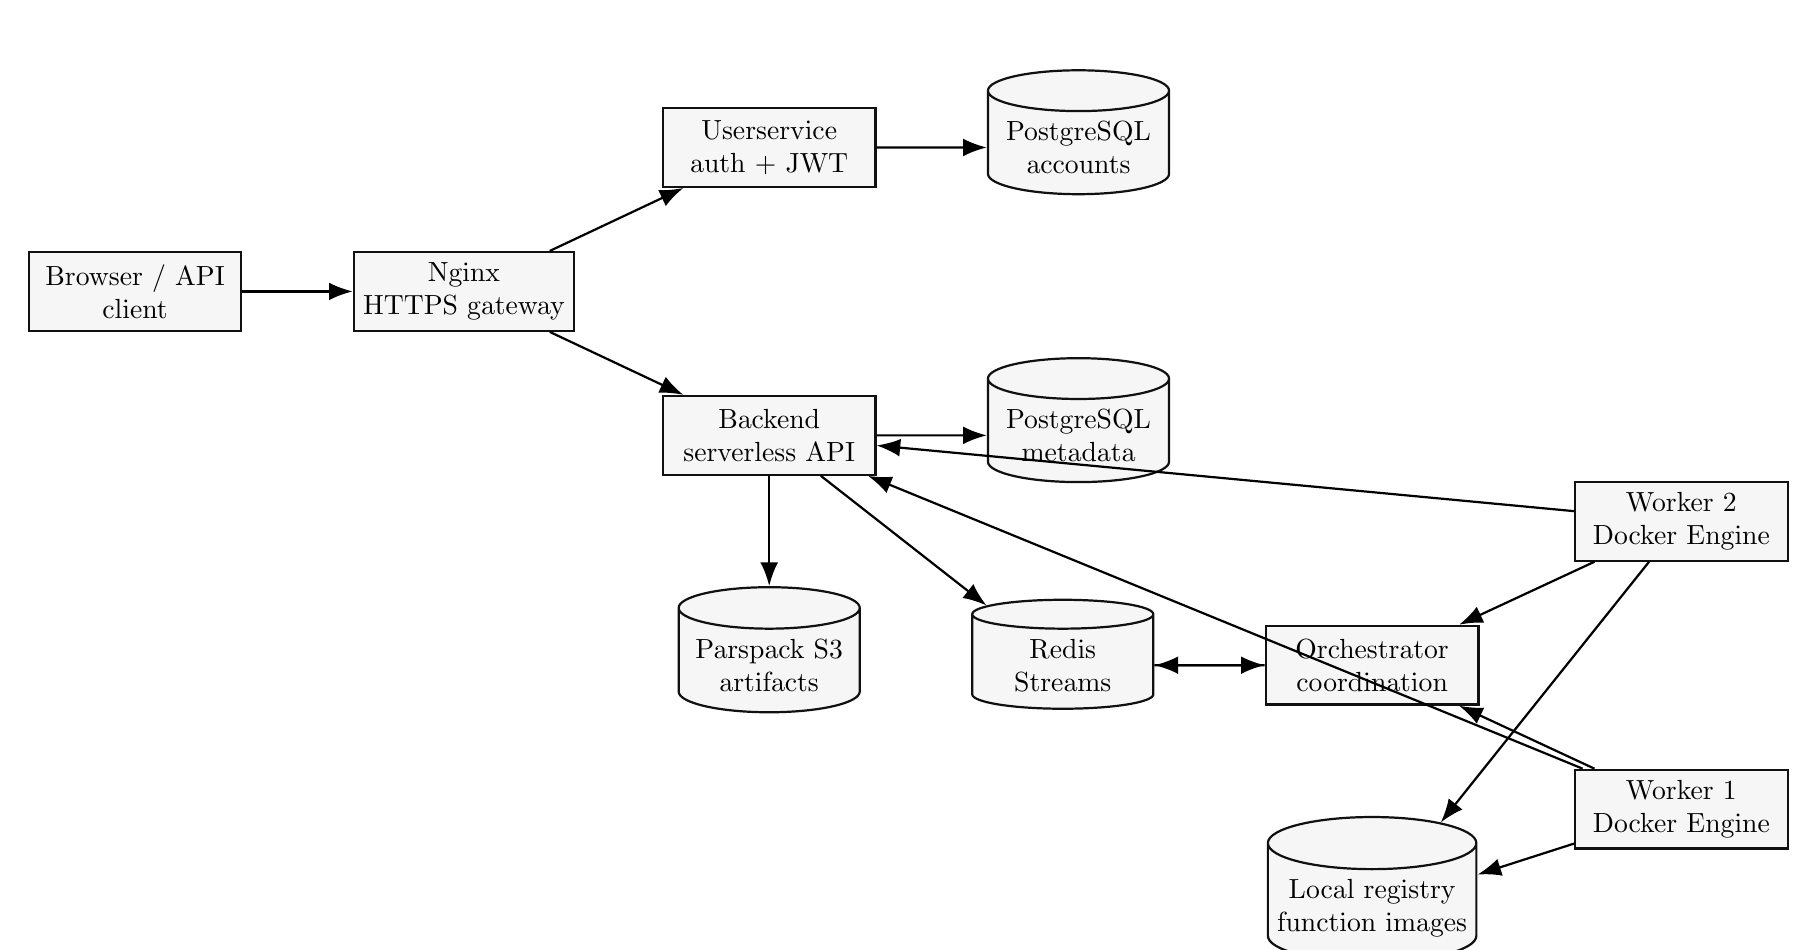
\begin{tikzpicture}[node distance=1.4cm]
  \node[svc] (client) {Browser / API\\client};
  \node[svc, right=of client] (nginx) {Nginx\\HTTPS gateway};
  \node[svc, below right=0.8cm and 1.1cm of nginx] (backend) {Backend\\serverless API};
  \node[svc, above right=0.8cm and 1.1cm of nginx] (user) {Userservice\\auth + JWT};
  \node[store, right=of backend] (pg) {PostgreSQL\\metadata};
  \node[store, right=of user] (userpg) {PostgreSQL\\accounts};
  \node[store, below=of backend] (storage) {Parspack S3\\artifacts};
  \node[store, right=of storage] (redis) {Redis\\Streams};
  \node[svc, right=of redis] (orch) {Orchestrator\\coordination};
  \node[svc, below right=0.8cm and 1.2cm of orch] (w1) {Worker 1\\Docker Engine};
  \node[svc, above right=0.8cm and 1.2cm of orch] (w2) {Worker 2\\Docker Engine};
  \node[store, below=of orch] (registry) {Local registry\\function images};

  \draw[arrow] (client) -- (nginx);
  \draw[arrow] (nginx) -- (backend);
  \draw[arrow] (nginx) -- (user);
  \draw[arrow] (backend) -- (pg);
  \draw[arrow] (user) -- (userpg);
  \draw[arrow] (backend) -- (storage);
  \draw[arrow] (backend) -- (redis);
  \draw[arrow] (redis) -- (orch);
  \draw[arrow] (orch) -- (redis);
  \draw[arrow] (w1) -- (backend);
  \draw[arrow] (w2) -- (backend);
  \draw[arrow] (w1) -- (orch);
  \draw[arrow] (w2) -- (orch);
  \draw[arrow] (w1) -- (registry);
  \draw[arrow] (w2) -- (registry);
\end{tikzpicture}
}
\caption{Current distributed prototype topology.}
\end{figure}

\clearpage

\chapter{Using the Platform}

\section{Mental model for users}

A user works with four main concepts:

\begin{description}[leftmargin=2.8cm,style=nextline]
  \item[Function] A named Python unit owned by a user.
  \item[Source] The function code, dependencies, handler setting, and contract.
  \item[Build] A Docker image produced from the source.
  \item[Invocation] One request to run a built function with a specific event and optional files.
\end{description}

The function source must define a handler. A simple handler looks like this:

\begin{lstlisting}[language=Python,caption={Minimal Python handler.}]
def main(event, context):
    name = event.get("name", "world")
    return {"message": f"Hello, {name}!"}
\end{lstlisting}

The handler receives two arguments. The \file{event} argument is the JSON
payload supplied by the caller. The \file{context} argument contains platform
metadata such as the request identifier and paths for input and output files.

\section{Source and dependency specification}

The frontend lets users paste the main handler code and \file{requirements.txt}.
Internally the platform packages those files into a ZIP source bundle. The
worker turns that bundle into a Docker image. The image build uses the declared
runtime, currently Python 3.13 in the common path.

\begin{lstlisting}[language=bash,caption={Example requirements.txt.}]
requests==2.32.3
numpy==2.2.0
\end{lstlisting}

Dependency builds are one of the areas where the prototype is useful but not
yet complete. Pure Python packages are straightforward. Packages with compiled
wheels or system-level dependencies may require extra build image support.
Future work should include runtime base image variants, build templates, or a
controlled mechanism for system packages.

\section{Access modes}

Each function has an invocation access mode:

\begin{itemize}[leftmargin=1.2cm]
  \item \state{private}: only the owner or an admin can invoke with a JWT.
  \item \state{token}: callers invoke with \api{X-Function-Token}.
  \item \state{public}: callers can invoke without JWT or function token.
\end{itemize}

Function tokens are intentionally not JWTs. A JWT proves account identity. A
function invocation token proves permission to call one function. This makes it
possible to rotate or revoke function access without changing account login
tokens.

\section{Asynchronous invocation}

Asynchronous invocation is the main durable execution path. It supports file
inputs, declared output files, polling, and ZIP download. The first response
returns an invocation identifier and a read token. The caller polls the
invocation endpoint until the invocation reaches a terminal state.

\begin{lstlisting}[language=bash,caption={Asynchronous invocation example.}]
curl -X POST https://fleetingcircus.ir/api/functions/42/invoke/ \
  -H "Authorization: Bearer <jwt>" \
  -H "Content-Type: application/json" \
  -d '{"event":{"name":"Ilya","numbers":[1,2,3]}}'
\end{lstlisting}

A simple response mode is the default. It keeps the API response focused on
what most users want: status, returned result, and output paths. The advanced
mode includes more platform metadata for debugging and frontend diagnostics.

\section{Synchronous invocation}

Synchronous invocation is a convenience path for functions that are expected to
finish quickly and do not require file input or declared output files. It waits
for the result and returns it in the original HTTP response if the function
finishes within the synchronous wait budget. The function timeout is separate:
it counts only actual function execution time, not network delay, queueing
delay, or scheduling delay.

\begin{lstlisting}[language=bash,caption={Synchronous invocation example.}]
curl -X POST https://fleetingcircus.ir/api/functions/42/invoke-sync/ \
  -H "Authorization: Bearer <jwt>" \
  -H "Content-Type: application/json" \
  -d '{"event":{"x":10,"y":20},"response_mode":"simple"}'
\end{lstlisting}

\section{Downloading invocation artifacts}

For asynchronous invocations, the caller can download an invocation ZIP while
the invocation is still retained. The retention rule for the prototype is that
invocations, their inputs, outputs, and logs expire together after seven days.
Expired invocations return HTTP 404 as if they never existed.

The ZIP contains a reference to the function and version, the original input
files, declared output files, stdout, stderr, and result metadata. Source code
is not included in invocation downloads.

\clearpage

\chapter{Architecture}

\section{Service responsibilities}

The architecture is deliberately split into services even though this is still
a prototype. The separation reflects the direction of the system:

\begin{longtable}{p{0.28\textwidth}p{0.68\textwidth}}
\toprule
\textbf{Service} & \textbf{Responsibility} \\
\midrule
\service{userservice} & Owns account data, password handling, JWT issuing, refresh, role claims, and public key/JWKS discovery. \\
\service{backend} & Owns the product API: functions, source bundles, builds, invocations, tokens, artifacts, downloads, OpenAPI, and ownership checks. \\
\service{orchestrator} & Owns V2 active coordination state in Redis: dispatch, claim, leases, completion acceptance, recovery, and final state transitions. \\
\service{worker} & Performs Docker image builds and function execution. Maintains local warm containers and reports state. \\
\service{invocation-finalizer} & Commits staged invocation artifacts and moves accepted completions into visible terminal results. \\
\service{projector} & Projects orchestrator events into PostgreSQL so user-facing history remains queryable. \\
\service{cleaners} & Clean expired invocations, staged artifacts, dead-letter records, and registry images marked for deletion. \\
\bottomrule
\end{longtable}

This split was not present at the very beginning. The first implementation was
closer to a Django backend that directly queued and coordinated jobs. As the
prototype moved toward multiple workers and reliability, the coordination logic
was moved toward an orchestrator role.

\section{Data stores}

\subsection{PostgreSQL}

PostgreSQL stores persistent platform metadata. It is the long-term record for
functions, versions, build attempts, invocation records, output metadata, log
artifact pointers, ownership, and history projections. It is not the fastest
possible coordination store, but it is reliable and easy to query.

\subsection{Redis}

Redis is used for active job coordination. The current V2 path uses Redis
Streams and Redis keys for job state, worker leases, dispatch attempts,
finalization markers, recovery sets, and worker metrics. Redis is faster than
PostgreSQL for small coordination transitions and queue operations. It also
allows the orchestrator to process jobs without performing a PostgreSQL query
for every small state change.

\subsection{Object storage}

Media artifacts are stored through Django's storage interface. The deployed
prototype now uses Parspack S3-compatible object storage. This is used for
source bundles, invocation inputs, output files, logs, and invocation ZIPs.
Before object storage was enabled on the deployed control plane, artifacts were
stored in the local backend media volume; old artifacts were not migrated.

Object storage is not a finalization-only dependency. It appears in several
parts of the lifecycle:

\begin{enumerate}[leftmargin=1.2cm]
  \item During function upload, the backend stores the source bundle.
  \item During asynchronous invocation, the backend stores uploaded input files.
  \item During execution, declared outputs may be uploaded directly by the runner or indirectly by the worker as staged artifacts.
  \item During finalization, the backend verifies staged artifact metadata and marks the accepted files as committed.
  \item During result download, the backend reads committed files and logs to produce the invocation ZIP.
\end{enumerate}

The orchestrator does not read or write object bytes. It only stores and checks
metadata: job IDs, attempts, completion IDs, terminal state, and artifact
commit IDs. This is why object-storage failures should surface as artifact
staging or finalization failures, not as scheduler-placement failures.

\section{Why a separate userservice exists}

The userservice was separated because authentication should not be tied to the
load of function invocation and build traffic. If the serverless backend is
busy, slow, or being restarted, users should still be able to log in, refresh
tokens, and manage their account. The userservice signs RS256 JWTs. The backend
verifies them locally by using the userservice public key or JWKS endpoint, so
normal backend requests do not require a network call back to the userservice.

\clearpage

\chapter{Job Model and Orchestration}

\section{Why orchestration became necessary}

The earliest design could push work straight from the backend to Redis and let
workers consume it. That works for a tiny prototype, but it becomes fragile as
soon as the system needs multiple workers, retries, recovery, cancellation,
fairness between builds and invocations, and visibility into queue state.

The orchestrator exists because the backend should behave more like a product
API gateway and less like the active scheduler. The orchestrator owns the
fast-changing coordination state. It chooses workers, grants leases, fences
attempts, accepts completions, and recovers abandoned jobs.

\section{Coordination versions}

The project went through a V1 and V2 coordination model.

\begin{description}[leftmargin=2.6cm,style=nextline]
  \item[V1] PostgreSQL job rows were the main coordination authority. Redis
  Lists carried job IDs to queues. Dispatch, claim, running, recovery, and
  final reports passed through the backend.
  \item[V2] Redis Streams and orchestrator-owned state became the active
  authority. PostgreSQL remains a durable read model and history store through
  projection.
\end{description}

V1 is deprecated. It is kept only as compatibility code during the transition.
New development should focus on V2.

\section{V2 job state}

A V2 job follows a fenced state machine. The important states are:

\begin{itemize}[leftmargin=1.2cm]
  \item \state{queued}: job exists and is ready for placement.
  \item \state{dispatched}: orchestrator assigned it to a worker and attempt.
  \item \state{running}: worker successfully claimed the delivery.
  \item \state{recovering}: lease expired or delivery needs repair.
  \item \state{finalizing}: worker has finished and completion was accepted, but artifacts are not yet committed.
  \item \state{succeeded}, \state{failed}, \state{cancelled}, \state{dead\_lettered}: terminal states.
\end{itemize}

The \file{dispatch\_attempt} number is a fencing token. If a worker reports
completion for an old attempt after the job was recovered and redispatched, the
orchestrator rejects the stale report.

\begin{figure}[h]
\centering
\resizebox{\textwidth}{!}{%
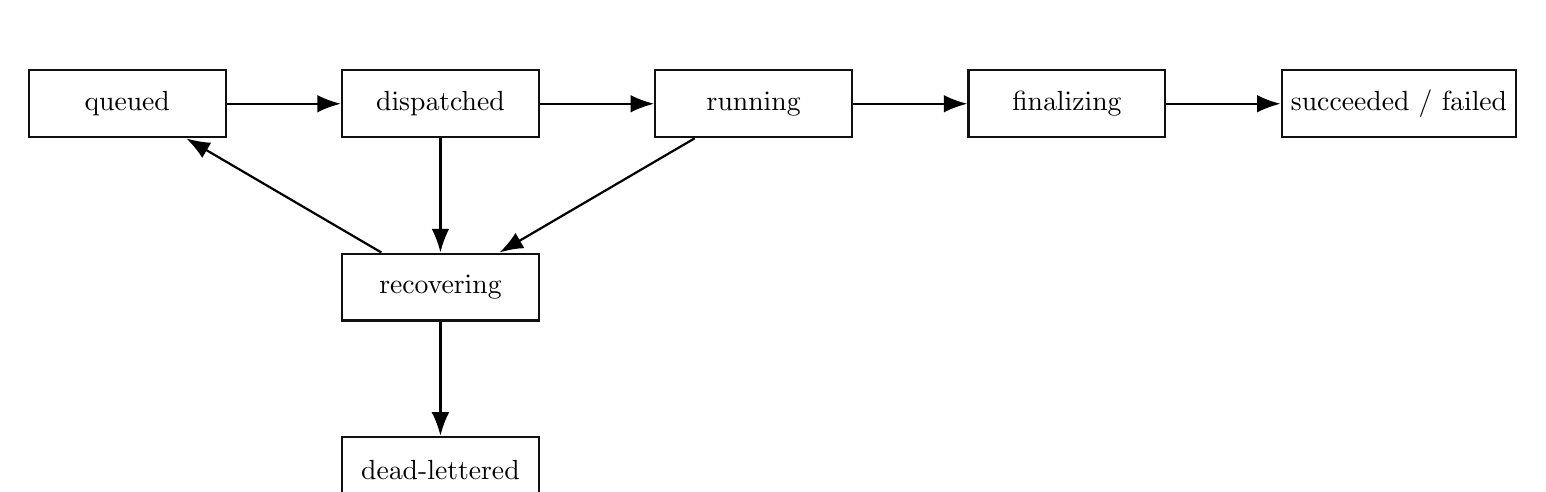
\begin{tikzpicture}[node distance=1.45cm]
  \node[queue] (q) {queued};
  \node[queue, right=of q] (d) {dispatched};
  \node[queue, right=of d] (r) {running};
  \node[queue, right=of r] (f) {finalizing};
  \node[queue, right=of f] (s) {succeeded / failed};
  \node[queue, below=of d] (rec) {recovering};
  \node[queue, below=of rec] (dead) {dead-lettered};
  \draw[arrow] (q) -- (d);
  \draw[arrow] (d) -- (r);
  \draw[arrow] (r) -- (f);
  \draw[arrow] (f) -- (s);
  \draw[arrow] (d) -- (rec);
  \draw[arrow] (r) -- (rec);
  \draw[arrow] (rec) -- (q);
  \draw[arrow] (rec) -- (dead);
\end{tikzpicture}}
\caption{Simplified V2 job state machine.}
\end{figure}

\section{Why Redis Streams}

Redis Streams were chosen instead of Pub/Sub because messages must survive
temporary consumer failure. Pub/Sub is transient: if a consumer is offline when
a message is published, the message is gone. Streams keep messages until they
are acknowledged or trimmed. Consumer groups also expose pending entries, which
lets the orchestrator and background services recover work after crashes.

\section{Backoff and dead-letter behavior}

Recovery is not allowed to retry forever. If a job keeps being redispatched and
recovered, it eventually becomes \state{dead\_lettered}. This protects the
platform from jobs that repeatedly fail because of a broken worker, bad image,
or persistent infrastructure issue.

Backoff delays are different for builds and invocations. Builds are expensive
and users tolerate a longer delay, so build recovery can wait longer between
attempts. Invocations are more user-visible, so their retry delays start faster.
The prototype uses this policy direction because it matches the product
expectation: invocation latency matters more than build latency, while build
storms can damage worker capacity.

\clearpage

\chapter{Build Flow}

\section{Build overview}

The build path converts user source into a runnable Docker image. A function
can have only one active build in the current product semantics. If the user
changes source code, the new source creates a replacement build. The old active
image continues serving until the new build succeeds. If the new build fails,
the existing active image stays active.

\begin{figure}[h]
\centering
\resizebox{\textwidth}{!}{%
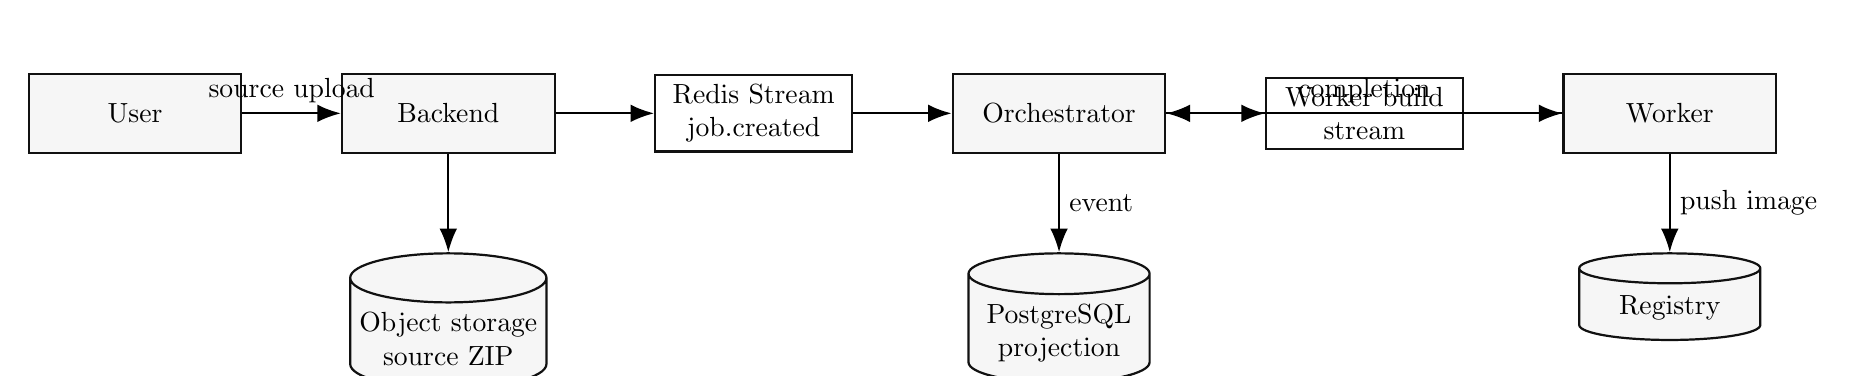
\begin{tikzpicture}[node distance=1.25cm]
  \node[svc] (user) {User};
  \node[svc, right=of user] (backend) {Backend};
  \node[store, below=of backend] (storage) {Object storage\\source ZIP};
  \node[queue, right=of backend] (stream) {Redis Stream\\job.created};
  \node[svc, right=of stream] (orch) {Orchestrator};
  \node[queue, right=of orch] (wq) {Worker build\\stream};
  \node[svc, right=of wq] (worker) {Worker};
  \node[store, below=of worker] (registry) {Registry};
  \node[store, below=of orch] (pg) {PostgreSQL\\projection};
  \draw[arrow] (user) -- node[above]{source upload} (backend);
  \draw[arrow] (backend) -- (storage);
  \draw[arrow] (backend) -- (stream);
  \draw[arrow] (stream) -- (orch);
  \draw[arrow] (orch) -- (wq);
  \draw[arrow] (wq) -- (worker);
  \draw[arrow] (worker) -- node[right]{push image} (registry);
  \draw[arrow] (worker) -- node[above]{completion} (orch);
  \draw[arrow] (orch) -- node[right]{event} (pg);
\end{tikzpicture}}
\caption{Build job flow.}
\end{figure}

\section{Source bundle}

The uploaded source bundle contains at least:

\begin{itemize}[leftmargin=1.2cm]
  \item \file{handler.py}
  \item \file{requirements.txt}
  \item \file{config.json}
\end{itemize}

The backend validates the bundle before storing it. Unsafe paths are rejected.
That means entries such as absolute paths or parent-directory traversal are not
allowed. This protects the builder from source bundles that try to write
outside the expected build context.

\section{Builder output}

The worker builder generates a small runtime wrapper and Dockerfile. The
runner imports the handler, loads the event, calls the function, writes the
JSON result, and captures stdout/stderr through Docker logs and artifact files.

\begin{lstlisting}[language=Python,caption={Simplified runner behavior.}]
handler_path = os.environ["FUNCTION_HANDLER"]  # for example: handler.main
module_name, function_name = handler_path.rsplit(".", 1)

module = importlib.import_module(module_name)
handler = getattr(module, function_name)

with open(os.environ["FUNCTION_EVENT_PATH"], "r", encoding="utf-8") as f:
    event = json.load(f)

context = {
    "request_id": os.environ.get("FUNCTION_REQUEST_ID"),
    "input_dir": os.environ.get("FUNCTION_INPUT_FILES_DIR"),
    "output_dir": os.environ.get("FUNCTION_OUTPUT_DIR"),
}

result = handler(event, context)

with open(os.path.join(context["output_dir"], "result.json"), "w") as f:
    json.dump(result, f)
\end{lstlisting}

The real runner contains more detail, including timing measurements, direct
output upload support, and reserved file handling. The snippet above captures
the core idea.

\section{Build image lifecycle}

Build output images are stored in a local Docker registry. In the current
distributed deployment, the control plane hosts the registry and workers pull
from it over the private network. Function image records track whether an image
is active, superseded, failed, pending deletion, deleted, or delete-failed. This
ledger matters because image deletion must not accidentally remove the active
image for a function.

\section{Build cancellation and retry}

Build jobs support queued cancellation and cooperative running cancellation.
The admin can configure a build retry policy. Per-attempt build history is
stored so that a failed build can be examined without losing the overall build
state. The current prototype has the policy mechanics; production-level build
resource isolation and package scanning remain future work.

\clearpage

\chapter{Invocation Flow in Detail}

\section{Asynchronous invocation, step by step}

An asynchronous invocation is the most complete and important path in the
system. It is designed for JSON events, optional input files, declared output
files, durable polling, and artifact download.

\begin{enumerate}[leftmargin=1.2cm]
  \item The caller sends \api{POST /api/functions/\{id\}/invoke/}.
  \item The backend authenticates the caller through JWT, function token, or public access.
  \item The backend selects the active built function version.
  \item The backend validates the JSON event and any input files.
  \item Input files are stored as invocation input artifact records.
  \item The backend creates an invocation record and a durable job creation event.
  \item The outbox relay publishes the creation event to Redis.
  \item The orchestrator reads the event and places the job on a worker stream.
  \item The worker consumes the delivery and asks the orchestrator to claim it.
  \item The orchestrator verifies the worker name, attempt, state, and lease.
  \item The worker fetches payload and input files from protected backend endpoints.
  \item The worker prepares a sandbox and runs or reuses a function container.
  \item The runner loads the event and calls the handler.
	
  \item The finalizer asks the backend to commit the staged artifacts.
  \item The backend makes artifacts visible only after verification and commit.
  \item The orchestrator records terminal state and emits a projection event.
  \item The projector updates PostgreSQL history.
  \item The caller polls the invocation endpoint and sees the final result.
\end{enumerate}

\section{Invocation execution diagram}

\begin{figure}[h]
\centering
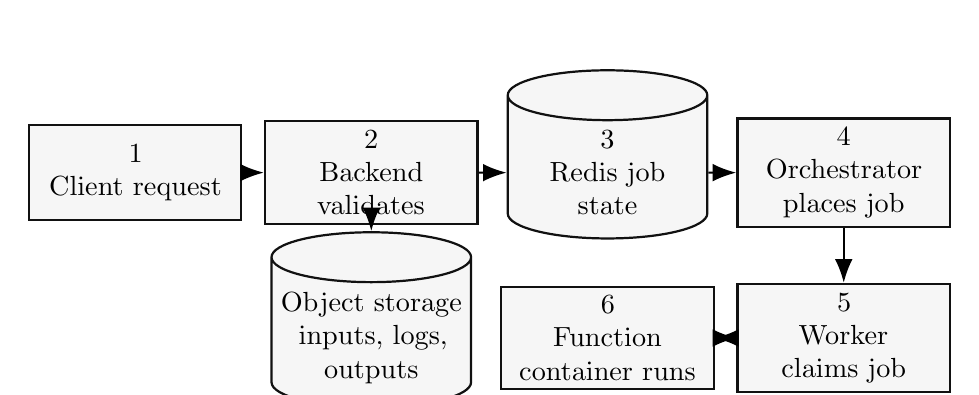
\begin{tikzpicture}[
  stage/.style={svc, text width=2.3cm, minimum height=1.2cm, align=center},
  storestage/.style={store, text width=2.3cm, minimum height=1.2cm, align=center}
]
  \node[stage] (client) at (0,0) {1\\Client request};
  \node[stage] (backend) at (3,0) {2\\Backend validates};
  \node[storestage] (storage) at (3,-2.1) {Object storage\\inputs, logs, outputs};
  \node[storestage] (redis) at (6,0) {3\\Redis job state};
  \node[stage] (orch) at (9,0) {4\\Orchestrator places job};
  \node[stage] (worker) at (9,-2.1) {5\\Worker claims job};
  \node[stage] (container) at (6,-2.1) {6\\Function container runs};

  \draw[arrow] (client) -- (backend);
  \draw[arrow] (backend) -- (redis);
  \draw[arrow] (redis) -- (orch);
  \draw[arrow] (orch) -- (worker);
  \draw[arrow] (worker) -- (container);
  \draw[arrow] (container) -- (worker);
  \draw[arrow] (backend) -- (storage);
\end{tikzpicture}
\caption{Asynchronous invocation execution path. The backend owns artifact storage. The orchestrator owns Redis coordination. The worker runs the function and reports completion.}
\end{figure}

The important boundary is that artifact bytes do not pass through the
orchestrator. Inputs, staged outputs, logs, and ZIP material are handled by
backend-owned artifact APIs and object storage. The orchestrator only sees job
metadata, attempts, leases, completion IDs, terminal status, and manifests.

\section{Finalization and projection diagram}

\begin{figure}[h]
\centering
\resizebox{\textwidth}{!}{%
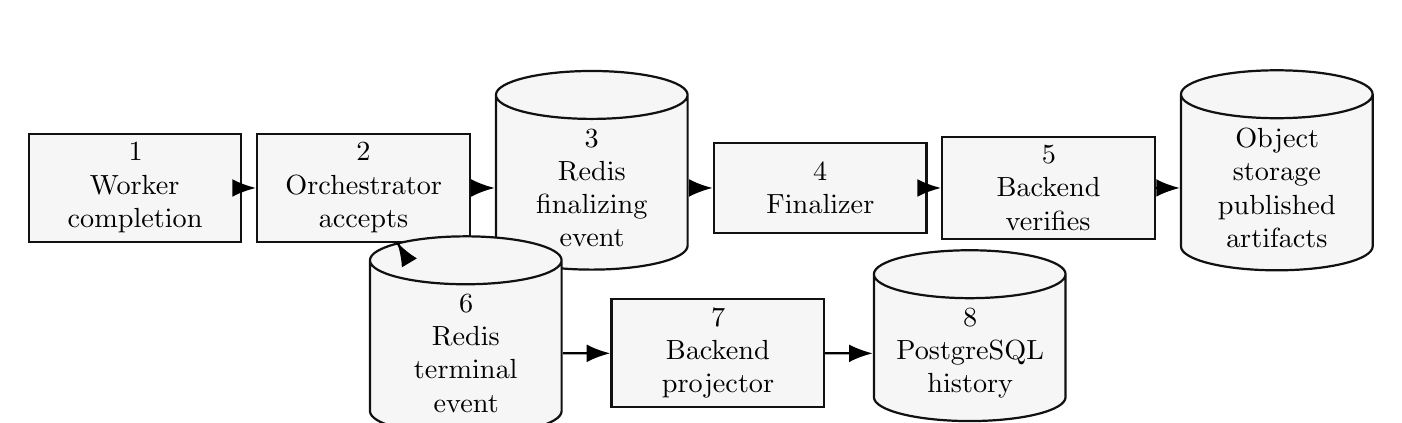
\begin{tikzpicture}[
  stage/.style={svc, text width=2.15cm, minimum height=1.15cm, align=center},
  storestage/.style={store, text width=2.2cm, minimum height=1.15cm, align=center}
]
  \node[stage] (worker) at (0,0) {1\\Worker completion};
  \node[stage] (orch1) at (2.9,0) {2\\Orchestrator accepts};
  \node[storestage] (redis1) at (5.8,0) {3\\Redis finalizing event};
  \node[stage] (finalizer) at (8.7,0) {4\\Finalizer};
  \node[stage] (backend) at (11.6,0) {5\\Backend verifies};
  \node[storestage] (storage) at (14.5,0) {Object storage\\published artifacts};

  \node[storestage] (redis2) at (4.2,-2.1) {6\\Redis terminal event};
  \node[stage] (projector) at (7.4,-2.1) {7\\Backend projector};
  \node[storestage] (pg) at (10.6,-2.1) {8\\PostgreSQL history};

  \draw[arrow] (worker) -- (orch1);
  \draw[arrow] (orch1) -- (redis1);
  \draw[arrow] (redis1) -- (finalizer);
  \draw[arrow] (finalizer) -- (backend);
  \draw[arrow] (backend) -- (storage);
  \draw[arrow] (orch1) -- (redis2);
  \draw[arrow] (redis2) -- (projector);
  \draw[arrow] (projector) -- (pg);
\end{tikzpicture}}
\caption{Finalization and projection path. The orchestrator does not write PostgreSQL directly; it emits Redis projection events consumed by the backend projector.}
\end{figure}

The finalizer is not the only component that can cause object-storage traffic.
It is shown here only because it is responsible for committing already staged
artifacts after the worker has finished executing. Earlier storage operations,
such as source uploads and input uploads, are handled by the backend before the
finalizer becomes involved.

\section{Input sandbox}

Input files are not simply mounted from arbitrary user paths. The backend
stores uploaded input files, and the worker downloads them through internal
endpoints. The worker writes sanitized copies into a temporary sandbox. The
function receives a directory path and a metadata JSON value so that it can
open the files explicitly.

This design has overhead: files are uploaded to the backend, persisted, fetched
by the worker, and copied into the sandbox. The tradeoff is that the platform
owns validation, retention, download behavior, and access control.

\section{Output sandbox}

The function writes declared output files into \file{/sandbox/output}. The
prototype has experimented with several strategies for collecting outputs:

\begin{itemize}[leftmargin=1.2cm]
  \item normal Docker volumes,
  \item tmpfs output mounts with size limits,
  \item Docker export/copy after execution,
  \item direct runner upload to the backend.
\end{itemize}

The current direction is performance-oriented: if no declared output files
exist, output export is skipped. This matters because Docker archive and copy
operations were visible in the timing reports even when the user function was
small. Avoiding that work on the common JSON-only path is one of the simplest
latency wins.

For output-producing invocations, the current implementation has two paths. The
preferred fast path is direct runner upload. The worker starts the function
container with scoped upload metadata in environment variables: upload URL,
upload token, job ID, dispatch attempt, completion ID, declared output names,
and byte limits. That data is not general backend access. It is permission to
upload staged outputs for exactly one fenced execution attempt.

The following excerpt is from \file{worker/builder.py}. This is more useful
than pseudocode because it shows the exact boundary between ``a function wrote a
file'' and ``the platform accepts this as a staged output''. The runner refuses
to use direct upload unless every fencing field is present, reads the declared
contract from the environment, scans the output directory, uploads accepted
files, and returns a manifest. If the runner cannot produce a manifest for a
function that declares outputs, the worker treats the invocation as failed.

\begin{lstlisting}[language=Python,caption={Direct runner upload gate from worker/builder.py.}]
def upload_declared_outputs_directly(output_dir, timings, env=None):
    if output_dir is None or not truthy(env_get(env, "FUNCTION_OUTPUT_DIRECT_UPLOAD_ENABLED")):
        return None

    upload_url = env_get(env, "FUNCTION_OUTPUT_UPLOAD_URL", "")
    upload_token = env_get(env, "FUNCTION_OUTPUT_UPLOAD_TOKEN", "")
    job_id = env_get(env, "FUNCTION_OUTPUT_UPLOAD_JOB_ID", "")
    completion_id = env_get(env, "FUNCTION_OUTPUT_UPLOAD_COMPLETION_ID", "")
    dispatch_attempt = int_env("FUNCTION_OUTPUT_UPLOAD_DISPATCH_ATTEMPT", 0, env=env)
    timeout = int_env("FUNCTION_OUTPUT_UPLOAD_TIMEOUT_SECONDS", 10, env=env)
    if not upload_url or not upload_token or not job_id or not completion_id or dispatch_attempt < 1:
        raise RuntimeError("Direct output upload is enabled but upload metadata is incomplete.")

    scan_started = time.perf_counter_ns()
    declared = json.loads(env_get(env, "FUNCTION_DECLARED_OUTPUT_FILES", "[]") or "[]")
    output_files = collect_declared_output_files(
        output_dir,
        declared,
        int_env("FUNCTION_OUTPUT_MAX_FILES", len(declared), env=env),
        int_env("FUNCTION_OUTPUT_MAX_FILE_SIZE_BYTES", 10 * 1024 * 1024, env=env),
        int_env("FUNCTION_OUTPUT_MAX_TOTAL_SIZE_BYTES", 25 * 1024 * 1024, env=env),
    )
    timings["runner_output_scan_ms"] = elapsed_ms(scan_started)

    upload_started = time.perf_counter_ns()
    manifest = [
        upload_file(upload_url, upload_token, job_id, dispatch_attempt,
                    completion_id, item, position, timeout)
        for position, item in enumerate(output_files)
    ]
    timings["runner_output_upload_ms"] = elapsed_ms(upload_started)
    return manifest
\end{lstlisting}

The worker then decides whether Docker filesystem export is needed at all. This
decision is one of the main performance details in the prototype. JSON-only
functions avoid export completely. Direct-upload functions also avoid export
because the runner already uploaded staged outputs from inside the container.
Only the conservative fallback path copies \file{/sandbox/export} out of Docker
and performs worker-side validation/upload.

\begin{lstlisting}[language=Python,caption={Worker output path selection from worker/executor.py.}]
declares_outputs = self._declares_output_files(job)
if direct_output_upload:
    result = self._read_result(None, stdout)
    output_manifest = self._read_runner_output_manifest(stdout)
    if output_manifest is None and (job.get("declared_output_files") or []):
        return ExecutionResult(
            status="failed",
            error_message="Runner did not report direct output uploads.",
            ...
        )
    output_manifest = output_manifest or []
    timing["docker_export_copy_ms"] = 0
    timing["output_validation_ms"] = 0
    timing["output_upload_ms"] = 0
elif not declares_outputs:
    result = self._read_result(None, stdout)
    output_manifest = []
    timing["docker_export_copy_ms"] = 0
    timing["output_validation_ms"] = 0
    timing["output_upload_ms"] = 0
else:
    self._copy_directory_from_container(container, SANDBOX_EXPORT_PATH, export_dir)
    output_files = self._validate_declared_output_files(job, effective_output_dir)
    output_manifest = self._upload_output_files(job, output_files)
\end{lstlisting}

The backend still remains the authority for visibility. Direct runner upload
does not mean ``the user can now download the file''. The upload endpoint first
verifies the runner upload token and the fenced attempt headers, then writes the
file as \state{staged}. Staged files physically exist but are not returned by
normal user-facing APIs.

\begin{lstlisting}[language=Python,caption={Direct staged-output upload endpoint from backend/apps/invocations/views.py.}]
token = request.headers.get("X-Runner-Upload-Token", "")
job_id = request.headers.get("X-Job-Id", "")
dispatch_attempt = int(request.headers.get("X-Dispatch-Attempt", "0") or 0)
completion_id = request.headers.get("X-Completion-Id", "")
original_path = request.headers.get("X-Original-Path", "")

verify_runner_output_upload_token(
    token,
    request_id=request_id,
    job_id=job_id,
    dispatch_attempt=dispatch_attempt,
    completion_id=completion_id,
)

uploaded_file = ContentFile(request.body or b"")
uploaded_file.name = original_path or "output"
uploaded_file.content_type = request.headers.get("Content-Type", "") or ""

output = store_staged_invocation_output_file(
    invocation=invocation,
    job_id=job_id,
    dispatch_attempt=dispatch_attempt,
    completion_id=completion_id,
    uploaded_file=uploaded_file,
    original_path=original_path,
    checksum_sha256="",
    position=position,
)
\end{lstlisting}

The final commit step is where staged artifacts become published artifacts. The
backend verifies that the manifest reported by the worker/orchestrator matches
the staged files already stored for that completion. Only then does it mark the
completion and output files as \state{committed}. The serializer later filters
on this committed state, which is why users cannot see half-finished outputs.

\begin{lstlisting}[language=Python,caption={Backend staged-artifact commit boundary from backend/apps/invocations/services.py.}]
files = list(completion.output_files.order_by("position", "id"))
verify_output_manifest(files, output_manifest)

completion.terminal_status = terminal_status
completion.result = completion_payload.get("result") or {}
completion.stdout = log_preview(completion_payload.get("stdout", ""))
completion.stderr = log_preview(completion_payload.get("stderr", ""))
completion.exit_code = completion_payload.get("exit_code")
completion.output_manifest = output_manifest
completion.artifact_commit_id = completion.artifact_commit_id or uuid.uuid4()
completion.status = StagedCompletionStatus.COMMITTED
completion.committed_at = timezone.now()
completion.save()

completion.output_files.update(status=StagedCompletionStatus.COMMITTED)
\end{lstlisting}

\section{Why staged artifacts exist}

Without staging, a bad failure order could expose partial output files before
the platform marks the invocation complete. Staging solves this. The worker
uploads outputs as invisible staged artifacts tied to one invocation, one
dispatch attempt, and one completion ID. Users cannot download them yet. Only
after the orchestrator accepts completion and the finalizer commits artifacts
do they become visible.

\begin{figure}[h]
\centering
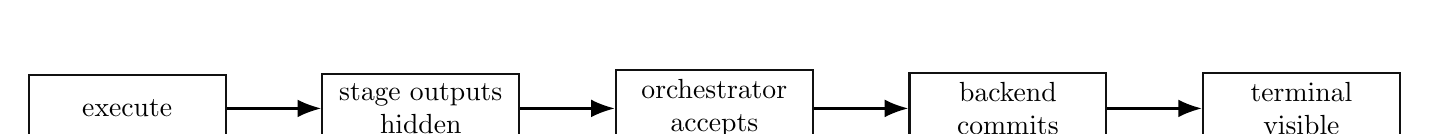
\begin{tikzpicture}[node distance=1.2cm]
  \node[queue] (exec) {execute};
  \node[queue, right=of exec] (stage) {stage outputs\\hidden};
  \node[queue, right=of stage] (accept) {orchestrator\\accepts};
  \node[queue, right=of accept] (commit) {backend\\commits};
  \node[queue, right=of commit] (visible) {terminal\\visible};
  \draw[arrow] (exec) -- (stage);
  \draw[arrow] (stage) -- (accept);
  \draw[arrow] (accept) -- (commit);
  \draw[arrow] (commit) -- (visible);
\end{tikzpicture}
\caption{Staged artifact visibility rule.}
\end{figure}

\section{Simple and advanced response modes}

The default response mode is simple. Simple mode returns only the user-facing
information: status, result, and output paths. Advanced mode returns the richer
metadata already needed by debugging tools and the frontend.

\begin{lstlisting}[caption={Simple terminal invocation response.}]
{
  "status": "succeeded",
  "result": {"message": "Hello, Ilya!"},
  "outputs": [
    {
      "path": "report.txt",
      "download_url": "/api/invocations/9273/outputs/1480/download/"
    }
  ]
}
\end{lstlisting}

\clearpage

\chapter{The Worker and Function Containers}

\section{Worker responsibilities}

Workers are deliberately kept relatively simple. They do not own user accounts
or product metadata. Their job is to register, heartbeat, receive assigned
work, claim it, execute it, upload artifacts, and acknowledge the delivery only
after responsibility has safely moved forward.

Each worker has bounded concurrency. The important settings are:

\begin{itemize}[leftmargin=1.2cm]
  \item \file{WORKER\_MAX\_CONCURRENCY}: total jobs in flight.
  \item \file{WORKER\_MAX\_INVOCATION\_CONCURRENCY}: invocation jobs in flight.
  \item \file{WORKER\_MAX\_BUILD\_CONCURRENCY}: build jobs in flight.
\end{itemize}

The worker prioritizes invocations over builds. This matters because builds
can take much longer and should not cause short function calls to sit behind a
large dependency installation.

\section{Worker heartbeat}

Workers send heartbeats containing worker identity, status, active job counts,
queue names, and warm-container inventory. The scheduler/orchestrator uses this
information to avoid dead workers, avoid workers with active builds for
invocations, and route warm invocations when possible.

\begin{lstlisting}[caption={Simplified worker heartbeat data.}]
{
  "worker": "worker-1",
  "status": "online",
  "active_jobs": 3,
  "active_invocations": 3,
  "active_builds": 0,
  "max_invocation_concurrency": 12,
  "warm_containers": [
    {"function_version_id": 87, "idle": true, "last_used": 1788332000}
  ]
}
\end{lstlisting}

\section{Container create versus start}

Docker container creation and container start are separate phases. Creation
constructs a stopped container: filesystem layers are prepared, mounts are
attached, limits are configured, environment variables are set, and metadata is
registered with Docker. Starting the container begins execution of the process
inside the already-created container.

This distinction matters in benchmarks. Cold invocations pay both create and
start overhead. Warm containers avoid most repeated create/start cost, but they
must be reset carefully enough to avoid leaking state between invocations.

\section{Warm containers}

Warm containers were added because cold container execution was too expensive
for repeated small functions. The current warm-container design has these
stages:

\begin{itemize}[leftmargin=1.2cm]
  \item reactive warm containers only,
  \item one warm container per function version per worker by default,
  \item TTL-based eviction,
  \item scheduler-aware exact warm routing,
  \item guarded sticky routing as a fallback,
  \item usage- and pressure-aware eviction.
\end{itemize}

The most important performance improvement came from moving to a resident warm
runner. The old warm path still executed \file{python /runner.py} on each call.
The resident path starts a small runner server inside the warm container and
sends local requests to it. This avoids repeated Python startup and repeated
module imports for no-op or small functions.

\section{Warm container limitations}

A warm container for function version A cannot safely be used for function
version B. The image, dependencies, code, handler, environment, and possibly
module-level state are all specific to one function version. Reusing a warm
container across different functions would break isolation and correctness.

Warm containers also increase memory pressure. Keeping many containers alive
improves latency for repeated calls but consumes worker resources. That is why
the prototype uses TTL and pressure-aware eviction instead of keeping all warm
containers forever.

TTL means \emph{time to live}. In the warm-container pool, TTL is not a network
TTL. It is the maximum amount of time an idle warm container is allowed to sit
unused before the worker retires it. If a function is called repeatedly, the
container's \file{last\_used\_at} timestamp is refreshed on release. If nobody
uses it for \file{WORKER\_WARM\_IDLE\_TTL\_SECONDS}, the worker destroys it. In
the local benchmark profile this was tuned lower for faster feedback; in a
normal deployment it can be higher to keep frequently used functions warm.

The warm pool also has non-time-based retirement rules. A container can be
retired because it is too old, because it has served too many invocations, or
because a failed execution made it unsafe to reuse. These rules are deliberately
separate from TTL:

\begin{itemize}[leftmargin=1.2cm]
  \item idle TTL answers: ``has this idle container been unused too long?''
  \item maximum age answers: ``has this container existed too long overall?''
  \item maximum uses answers: ``has this container been reused enough times that refreshing it is safer?''
  \item failed execution answers: ``did the last run leave this container in an unknown state?''
\end{itemize}

Pressure-aware eviction is the part that decides what to remove when the pool
has too many containers. The pressure can come from three places: too many idle
containers for one function version, too many containers in the whole pool, or
too much warm-container memory reserved on that worker. This is better than
plain FIFO because FIFO might delete a useful hot container while keeping a
rarely used one. The implementation keeps per-container usage metadata and
chooses victims using hit count, use count, recency, age, and memory size.

\begin{lstlisting}[language=Python,caption={Warm-container retirement checks from worker/warm\_pool.py.}]
def _retirement_reason_locked(self, record):
    now = self._now()
    if self.idle_ttl_seconds and now - record.last_used_at >= self.idle_ttl_seconds:
        return "idle_ttl"
    if self.max_age_seconds and now - record.created_at >= self.max_age_seconds:
        return "max_age"
    if self.max_uses and record.use_count >= self.max_uses:
        return "max_uses"
    return ""
\end{lstlisting}

\begin{lstlisting}[language=Python,caption={Pressure-aware warm-pool victim selection from worker/warm\_pool.py.}]
def _choose_eviction_victim_locked(self, candidates, *, pressure):
    if pressure == "pool_memory_pressure":
        return min(candidates, key=lambda record: (
            record.hit_count,
            record.use_count,
            -record.key.memory_mb,
            record.last_used_at,
            record.created_at,
        ))
    return min(candidates, key=lambda record: (
        record.hit_count,
        record.use_count,
        record.last_used_at,
        record.created_at,
        -record.key.memory_mb,
    ))
\end{lstlisting}

The memory-pressure ordering intentionally treats large low-hit containers as
good eviction candidates. Under normal container-count pressure, the pool first
tries to remove low-hit, low-use, older idle containers. This is still a simple
policy, but it captures the important intuition: keep containers that are
actually being reused, and reclaim containers that are idle, cold in practice,
or expensive relative to their benefit.

\clearpage

\chapter{Scheduling Policy}

\section{What the orchestrator actually owns}

The current service is named \service{scheduler} in the repository, but its V2
role is closer to an orchestrator. It is responsible for fast-changing active
coordination state. It consumes V2 job creation events from Redis Streams,
creates Redis job-state hashes, places ready jobs onto worker-specific streams,
validates worker claims, grants leases, accepts completions, starts finalization
for invocation artifacts, marks build jobs terminal, recovers expired leases,
and emits projection events for PostgreSQL read models.

The orchestrator does not own source files, input files, output files, user
accounts, or function metadata. Those stay behind the backend and userservice.
The orchestrator owns the execution state machine. That distinction is
important: the backend is the product API; Redis plus the orchestrator are the
active control plane for V2 jobs.

\section{Job creation and ready set}

The backend creates a durable \state{job.created} event. The orchestrator
consumer reads that event from Redis, ignores non-V2 events, creates a Redis job
state, stores the payload, and inserts the job into a sorted ready set keyed by
\file{available\_at\_ms}. Delayed retries use the same ready set. A job is only
eligible for dispatch when its score is less than or equal to the current time.

\begin{lstlisting}[language=Python,caption={V2 job creation ingestion from scheduler/production\_orchestrator.py.}]
def process_creation_event(self, stream_id, fields):
    if fields.get("event_type") != "job.created":
        return False
    event = json.loads(fields["payload"])
    if int(event.get("coordination_version", 1)) != 2:
        return False

    job_id = str(event["job_id"])
    available_at_ms = timestamp_ms(event.get("available_at"))
    self.state.create_job(job_id, event["job_type"], available_at_ms=available_at_ms)
    self.redis.hset(self.state.key(job_id), mapping={
        "payload": json.dumps(event.get("payload") or {}, separators=(",", ":"),
                              sort_keys=True),
        "source_event_id": fields.get("event_id", ""),
        "source_stream_id": stream_id,
        "max_recovery_attempts": int(event.get("max_recovery_attempts", 3)),
    })
    self.redis.zadd(self.ready_key, {job_id: available_at_ms})
    return True
\end{lstlisting}

\section{Worker heartbeats as scheduling input}

Workers periodically report their current state. The orchestrator stores each
heartbeat in Redis and puts the worker name into a lease sorted set. If a worker
misses its heartbeat lease, \file{list\_online\_workers} expires it before
placement. This means the placement policy only sees workers that are currently
online according to Redis time and the configured worker lease TTL.

\begin{lstlisting}[language=Python,caption={Worker heartbeat fields from scheduler/orchestrator\_workers.py.}]
redis.call('HSET', KEYS[1],
    'name', ARGV[1],
    'hostname', ARGV[2],
    'status', ARGV[16],
    'max_concurrency', ARGV[3],
    'max_build_concurrency', ARGV[4],
    'max_invocation_concurrency', ARGV[5],
    'active_jobs', ARGV[6],
    'active_builds', ARGV[7],
    'active_invocations', ARGV[8],
    'metadata', ARGV[13],
    'last_seen_ms', ARGV[14],
    'lease_expires_at_ms', ARGV[15])
\end{lstlisting}

The \file{metadata} field includes warm-pool inventory. That is how the
orchestrator learns that a worker has, for example, an idle resident warm
container for function version 87 with a specific image, handler, memory limit,
and output tmpfs size. The orchestrator does not inspect Docker directly. It
trusts worker heartbeats as its worker-capacity view.

\section{Separate build and invocation streams}

V2 separates build and invocation deliveries. Each worker has a build stream and
an invocation stream. This prevents long build jobs from sitting directly in
front of latency-sensitive invocations. The worker loop also prioritizes
invocation stream reads when invocation capacity exists.

\begin{itemize}[leftmargin=1.2cm]
  \item job creation stream: backend-to-orchestrator events,
  \item ready sorted set: orchestrator-owned dispatch eligibility,
  \item worker invocation stream: V2 invocation deliveries for one worker,
  \item worker build stream: V2 build deliveries for one worker,
  \item finalization stream: invocation artifact commit work,
  \item projection stream: Redis terminal/running events copied to PostgreSQL.
\end{itemize}

\section{Invocation placement policy}

Invocation placement is more sophisticated than round robin. It uses reported
worker state plus short-lived local reservations inside the orchestrator
process. The local reservations matter because heartbeats are periodic. If the
orchestrator dispatches five jobs to the same worker between two heartbeats, the
worker's last reported \file{active\_jobs} may still look low. Local reservations
prevent the orchestrator from overbooking a worker before the next heartbeat
arrives.

The current invocation order is:

\begin{enumerate}[leftmargin=1.2cm]
  \item remove expired local dispatch reservations, warm reservations, and sticky routes;
  \item compute the exact warm-container key for the invocation;
  \item prefer online workers with no active or queued builds, available invocation capacity, and an exact idle warm container;
  \item if several warm workers match, choose the lowest invocation load and round-robin among ties;
  \item if no warm worker is visible, consider workers without active or queued builds;
  \item filter to workers below \file{max\_invocation\_concurrency} when possible;
  \item try guarded sticky routing only if the recently used worker is still capacity-safe;
  \item otherwise choose the least-loaded candidate and round-robin among ties.
\end{enumerate}

\begin{lstlisting}[language=Python,caption={Warm-first invocation placement from scheduler/scheduler.py.}]
warm_candidates = [
    worker
    for worker in workers
    if worker_active_builds(worker) == 0
    and worker_queued_builds(worker) == 0
    and invocation_load(worker, local_invocation_loads=local_invocation_loads,
                        local_load_ttl_seconds=local_load_ttl_seconds,
                        now=now) < worker_max_invocation_concurrency(worker)
    and worker_idle_warm_count(worker, warm_key,
                               local_warm_reservations=local_warm_reservations,
                               local_load_ttl_seconds=local_load_ttl_seconds,
                               now=now) > 0
]
if warm_candidates:
    best_load = min(invocation_load(worker, local_invocation_loads=local_invocation_loads,
                                    local_load_ttl_seconds=local_load_ttl_seconds,
                                    now=now)
                    for worker in warm_candidates)
    best = [worker for worker in warm_candidates
            if invocation_load(worker, local_invocation_loads=local_invocation_loads,
                               local_load_ttl_seconds=local_load_ttl_seconds,
                               now=now) == best_load]
    return choose_round_robin_worker(best, "warm-invocation", round_robin_state)
\end{lstlisting}

The warm key is intentionally exact. A warm container is only considered a match
when function version, image reference, handler, memory size, and output tmpfs
size match. A container for one function version cannot safely serve another
function version.

\begin{lstlisting}[language=Python,caption={Exact warm-container match from scheduler/scheduler.py.}]
return (
    str(item.get("function_version_id") or "")
    == str(warm_key.get("function_version_id") or "")
    and str(item.get("image_ref") or "") == str(warm_key.get("image_ref") or "")
    and str(item.get("handler") or "") == str(warm_key.get("handler") or "")
    and safe_int(item.get("memory_mb")) == safe_int(warm_key.get("memory_mb"))
    and safe_int(item.get("output_tmpfs_size_bytes"))
    == safe_int(warm_key.get("output_tmpfs_size_bytes"))
)
\end{lstlisting}

\section{Guarded sticky fallback}

Guarded sticky routing is a prediction layer, not the primary policy. It exists
because a worker may have created a warm container after a recent invocation,
but the next heartbeat may not have reported that warm container yet. The
orchestrator therefore remembers the recent route for a function version for a
short TTL, currently ten seconds in the policy path. It only follows that route
when the worker still has no build pressure, still has invocation capacity, and
is not much more loaded than the best reported candidate.

\begin{lstlisting}[language=Python,caption={Guarded sticky checks from scheduler/scheduler.py.}]
best_reported_load = min(worker_reported_invocation_load(worker)
                         for worker in candidates)
for worker in candidates:
    if worker.get("name") != worker_name:
        continue
    if worker_active_builds(worker) != 0 or worker_queued_builds(worker) != 0:
        return None
    reported_load = worker_reported_invocation_load(worker)
    local_dispatches = local_invocation_load(worker,
        local_invocation_loads=local_invocation_loads,
        local_load_ttl_seconds=local_load_ttl_seconds,
        now=now)
    if local_dispatches > predictive_sticky_max_local_dispatches:
        return None
    if reported_load + local_dispatches >= worker_max_invocation_concurrency(worker):
        return None
    if reported_load > best_reported_load + predictive_sticky_load_slack:
        return None
    return worker
\end{lstlisting}

The important parameters are not arbitrary adjectives. ``Capacity-safe'' means
reported active work plus locally remembered dispatches is below
\file{max\_invocation\_concurrency}. ``Not much more loaded'' means the sticky
worker's reported load is no more than \file{predictive\_sticky\_load\_slack}
above the best candidate's reported load. ``Local burst limit'' means the
orchestrator will not send more than
\file{predictive\_sticky\_max\_local\allowbreak\_dispatches} recent unconfirmed local
dispatches to the same sticky worker.

\section{Build placement policy}

Build placement is intentionally stricter than invocation placement. The build
selector only chooses workers with zero active jobs, zero queued invocations,
and zero queued builds. This protects the user-visible invocation path from
dependency installation and Docker build pressure. It can reduce build
throughput, but it gives the prototype a clearer latency priority.

\begin{lstlisting}[language=Python,caption={Build placement from scheduler/scheduler.py.}]
def choose_build_worker(workers, *, round_robin_state):
    candidates = [
        worker
        for worker in workers
        if worker_active_jobs(worker) == 0
        and worker_queued_invocations(worker) == 0
        and worker_queued_builds(worker) == 0
    ]
    if not candidates:
        return None
    return choose_round_robin_worker(candidates, "build", round_robin_state)
\end{lstlisting}

\section{Atomic dispatch}

After policy chooses a worker, dispatch must be atomic. It is not enough to set
\state{dispatched} and later push to a worker stream in separate operations,
because the orchestrator could crash between those operations. The production
orchestrator uses a Redis Lua script that checks the job is still queued,
increments \file{dispatch\_attempt}, writes assigned worker and lease metadata,
adds the delivery to the worker stream, stores the stream ID, and removes the
job from the ready set in one Redis operation.

\begin{lstlisting}[language=Python,caption={Atomic dispatch script from scheduler/production\_orchestrator.py.}]
local attempt = redis.call('HINCRBY', KEYS[1], 'dispatch_attempt', 1)
redis.call('HSET', KEYS[1],
    'status', 'dispatched',
    'assigned_worker', ARGV[1],
    'worker_stream', KEYS[3],
    'effective_image_ref', image_ref,
    'lease_expires_at_ms', ARGV[6],
    'updated_at_ms', ARGV[4])
local stream_id = redis.call('XADD', KEYS[3], '*',
    'job_id', ARGV[2],
    'dispatch_attempt', tostring(attempt),
    'job_type', ARGV[3])
redis.call('HSET', KEYS[1], 'delivery_stream_id', stream_id)
redis.call('ZREM', KEYS[2], ARGV[2])
return {'ok', 'dispatched', tostring(attempt), stream_id}
\end{lstlisting}

For build jobs, the dispatch script also creates an attempt-specific image tag.
The active function version is not switched to that image until the build
completes successfully and the terminal projection is committed. This prevents
a failed replacement build from breaking the currently working image.

\section{Claim and lease protocol}

Dispatch does not mean the worker may execute blindly. The worker reads a
delivery from its Redis Stream and calls the orchestrator claim API with
\file{worker\_name} and \file{dispatch\_attempt}. The orchestrator atomically
checks that the job is still assigned to that worker, that the attempt matches,
and that the job is still in \state{dispatched}. If the check passes, the job
moves to \state{running}, a lease expiry is written, and the orchestrator returns
the execution payload. If the check fails, the worker acknowledges the stale
delivery and does not execute it.

\begin{lstlisting}[language=Python,caption={Worker-side V2 claim before execution from worker/worker.py.}]
claim = orchestrator.claim_job(job_id, {
    "worker_name": worker_name,
    "dispatch_attempt": int(delivery.get("dispatch_attempt", 0)),
})
if not claim.get("claimed"):
    client.xack(worker_stream, V2_WORKER_GROUP, stream_id)
    continue

job = dict(claim.get("payload") or {})
pool.submit(run_v2_claimed_job, job=job, backend=backend,
            orchestrator=orchestrator, worker_name=worker_name, ...)
\end{lstlisting}

\begin{lstlisting}[language=Python,caption={Orchestrator claim transition from scheduler/orchestrator\_state.py.}]
local worker = redis.call('HGET', KEYS[1], 'assigned_worker') or ''
local attempt = tonumber(redis.call('HGET', KEYS[1], 'dispatch_attempt') or '0')
if worker ~= ARGV[1] or attempt ~= tonumber(ARGV[2]) then
    return {'stale', status, tostring(attempt)}
end
if status ~= 'dispatched' then
    return {'invalid_state', status, tostring(attempt)}
end
redis.call('HSET', KEYS[1],
    'status', 'running',
    'lease_expires_at_ms', ARGV[3],
    'updated_at_ms', ARGV[4])
return {'ok', 'running', tostring(attempt)}
\end{lstlisting}

The lease is renewed while the worker is executing. If the worker process dies,
the worker machine loses network connectivity, or the job stops renewing its
lease, the orchestrator can recover the job after the lease expires. The
dispatch attempt fencing token prevents an old worker from successfully
reporting completion after a newer attempt has already been created.

\section{Completion, finalization, and ACK}

For invocations, completion is split into two phases. First, the worker uploads
staged outputs and reports completion to the orchestrator. The orchestrator
verifies the worker and attempt, stores the completion payload in Redis, moves
the job to \state{finalizing}, removes the running lease, ACKs the worker
delivery, and emits a finalization event. At that point the function will not be
executed again for that attempt; responsibility has moved to the finalizer.

\begin{lstlisting}[language=Python,caption={Invocation completion acceptance from scheduler/production\_orchestrator.py.}]
begun = self.state.begin_finalization(
    job_id,
    worker_name=worker_name,
    dispatch_attempt=dispatch_attempt,
    completion_id=completion_id,
    completion_payload=completion_payload,
    terminal_status=status,
    now_ms=now_ms,
)
if job_before.get("job_type") == "invocation":
    self.redis.zrem(self.lease_key, job_id)
    self.ack_delivery(self.state.get_job(job_id))
    self.emit_finalization(job_id)
    return {"accepted": True, "status": V2JobStatus.FINALIZING, ...}
\end{lstlisting}

The finalizer later asks the backend to commit staged artifacts. After the
backend returns an \file{artifact\_commit\_id}, the finalizer calls the
orchestrator again. The orchestrator then moves \state{finalizing} to the
terminal state and emits a projection event. This second transition checks that
a successful invocation has an artifact commit ID; otherwise a succeeded result
would become visible without committed artifacts.

\begin{lstlisting}[language=Python,caption={Finalization guard from scheduler/orchestrator\_state.py.}]
if status ~= 'finalizing' then
    return {'invalid_state', status, tostring(attempt)}
end
if completion ~= ARGV[1] then
    return {'completion_conflict', status, tostring(attempt)}
end
if ARGV[2] == 'succeeded' and ARGV[3] == '' then
    return {'missing_artifact_commit', status, tostring(attempt)}
end
redis.call('HSET', KEYS[1],
    'status', ARGV[2],
    'artifact_commit_id', ARGV[3],
    'finished_at_ms', ARGV[4],
    'updated_at_ms', ARGV[4])
\end{lstlisting}

\section{Recovery and dead letters}

Recovery is driven by the orchestrator's job lease sorted set. When a dispatched
or running job's lease expires, the orchestrator checks its state. If the job
has not exceeded its maximum recovery count, it moves the job back to
\state{queued}, sets a future \file{available\_at\_ms} according to the backoff
policy, clears worker assignment fields, and redispatches it later. If it has
exceeded the configured recovery count, it becomes \state{dead\_lettered}. This
keeps the platform from retrying a permanently broken job forever.

\begin{lstlisting}[language=Python,caption={Recovery transition from scheduler/orchestrator\_state.py.}]
if attempt ~= tonumber(ARGV[1]) then
    return {'stale', status, tostring(attempt)}
end
local recovery = redis.call('HINCRBY', KEYS[1], 'recovery_count', 1)
redis.call('HSET', KEYS[1],
    'status', 'queued',
    'available_at_ms', ARGV[2],
    'last_error', ARGV[3],
    'updated_at_ms', ARGV[4])
redis.call('HDEL', KEYS[1],
    'assigned_worker', 'worker_queue', 'lease_expires_at_ms',
    'completion_id', 'completion_payload', 'completion_status',
    'artifact_commit_id')
\end{lstlisting}

\section{What can go wrong}

Scheduling is a balancing act. Too much stickiness can overload one worker
while others are idle. Too little stickiness causes repeated cold starts. Too
much build parallelism slows invocations. Too little build parallelism makes
builds wait unnecessarily. The current policy is practical but not final. Future
work can add richer signals such as recent CPU load, Docker daemon pressure,
image cache hits, per-function hotness, queue age, and per-worker p95 latency.

\clearpage

\chapter{Security and Access Control}

\section{Authentication}

Account authentication is handled by the userservice. It issues RS256 JWTs.
The backend validates those tokens locally using the public key/JWKS exposed by
the userservice. This avoids a network call for every authenticated backend
request.

\section{Authorization}

The backend enforces ownership rules for functions, versions, builds,
invocations, outputs, and token management. Admin users can access worker-node
management APIs. Internal worker and service endpoints use a shared internal
token through \api{X-Internal-Token}.

\section{Invocation tokens}

Invocation tokens are function-scoped opaque secrets. Creating or rotating a
token returns the raw token once. Later API responses only show metadata such
as token prefix, name, expiry, revoked state, and last-used time.

When an invocation is created by function token or public access, the platform
returns an invocation read token. This read token lets that caller poll and
download only the result of that specific invocation. A different token caller
should not be able to read another token caller's invocation output.

\section{Current hardening gaps}

The prototype is not yet hardened as a hostile multi-tenant platform. Important
future work includes CPU controls, process-count limits, read-only root
filesystems, seccomp/AppArmor profiles, stricter network controls, dependency
scanning, image scanning, and build isolation from the host Docker daemon.

\clearpage

\chapter{Artifacts, Logs, and Retention}

\section{Artifact categories}

The platform handles several artifact types:

\begin{itemize}[leftmargin=1.2cm]
  \item source bundles,
  \item invocation input files,
  \item invocation output files,
  \item stdout and stderr logs,
  \item invocation ZIP downloads,
  \item Docker images.
\end{itemize}

Source bundles are kept permanently according to the current project policy.
Invocation inputs, outputs, logs, and invocation records expire after seven
days. If an invocation expires, the API returns 404 as if the invocation never
existed.

\section{Log storage}

Logs are not stored as large database text fields. The current design stores
stdout and stderr as file artifacts, with database pointers and previews. This
avoids making PostgreSQL carry potentially large log bodies while still giving
the frontend enough information for status and basic display.

Full logs are included in the invocation ZIP. The user does not get separate
log browsing endpoints in the prototype UI contract.

\section{Object storage}

The deployed platform uses Parspack S3-compatible object storage for media
artifacts. The backend accesses it through Django storage, so most application
code uses the same file API whether storage is local or S3-backed.

This was recently verified with a public-domain smoke test. A function was
created, built, invoked, produced \file{report.txt}, and the backend confirmed
that both the output file and stdout log used \service{S3Storage} and existed
in the configured bucket.

\clearpage

\chapter{Reliability Design}

\section{Fencing tokens}

The platform uses dispatch attempts as fencing tokens. If a worker runs an old
delivery after recovery, its completion report contains the wrong attempt and
is rejected. This protects against stale workers overwriting newer state.

\section{Leases and recovery}

Dispatched and running V2 jobs hold leases. If the lease expires, recovery can
requeue the job or move it toward dead-letter depending on the recovery count.
The goal is to avoid permanent stuck jobs while also avoiding infinite retry
loops.

\section{Safe completion protocol}

The safe completion protocol avoids cross-database transactions between Redis
and PostgreSQL. Instead, it uses staging, idempotency, fencing, and retryable
finalization.

\begin{enumerate}[leftmargin=1.2cm]
  \item Worker uploads staged outputs.
  \item Worker reports completion with job ID, attempt, completion ID, status, result, and manifest.
  \item Orchestrator verifies running state and attempt, stores completion payload, moves to \state{finalizing}, and acknowledges worker delivery.
  \item Finalizer asks backend to commit staged artifacts.
  \item Backend verifies and marks artifacts committed in a transaction.
  \item Orchestrator verifies artifact commit ID and moves the job to terminal state.
  \item Projector records terminal history in PostgreSQL.
\end{enumerate}

The key rule is that a physical file may exist before the invocation is
terminal, but it is not visible to users until the final terminal transition.

\section{Graceful shutdown}

Workers support draining behavior. A draining worker should stop accepting new
work while letting in-flight jobs finish. This is necessary for maintenance,
deployments, and removing workers from the distributed deployment without
turning normal in-flight invocations into artificial failures.

\clearpage

\chapter{Observability}

\section{Stack}

The observability stack contains:

\begin{description}[leftmargin=3.0cm,style=nextline]
  \item[Prometheus] Scrapes and stores numeric metrics.
  \item[Grafana] Displays dashboards backed by Prometheus and Loki.
  \item[Loki] Stores searchable logs.
  \item[Grafana Alloy] Collects Docker logs from the control-plane host and ships them to Loki.
  \item[cAdvisor] Exposes container CPU, memory, filesystem, and network metrics.
  \item[Redis exporter] Exposes Redis metrics.
  \item[Postgres exporters] Expose backend and userservice database metrics.
\end{description}

The Grafana dashboard shows scrape health, worker reachability, queue backlog,
worker current state, queue pressure, worker execution, orchestrator stream
lag, finalization health, duplicate/fencing signals, storage-related errors,
and recent logs.

\section{Current observability limitation}

Loki currently collects control-plane Docker logs only. Worker metrics are
scraped from the worker VMs, but worker container logs are not shipped yet.
The next observability improvement should deploy Alloy or another log shipper
on each worker machine so that worker timing and failure logs appear in Loki.

\section{Interpreting empty panels}

An empty error panel does not necessarily mean observability is broken. It can
mean no error log line matched the filter in the selected time range. For this
reason, the dashboard includes a general recent platform logs panel. If normal
logs appear there but the error panel is empty, the system is observable and no
matching recent errors were found.

\clearpage

\chapter{Deployment}

\section{Local deployment}

The local deployment remains available through \file{docker-compose.yml}. It
is used for development and many of the repeatable tests.

\begin{lstlisting}[language=bash,caption={Local stack startup.}]
docker compose up -d
docker compose exec backend python manage.py migrate
docker compose exec userservice python manage.py migrate
\end{lstlisting}

\section{Distributed prototype deployment}

The first distributed deployment uses one control-plane machine and two worker
machines. The control plane hosts frontend, Nginx, userservice, backend,
PostgreSQL, Redis, registry, orchestrator services, finalizer, projector,
cleaners, and observability. Each worker machine runs a worker container and a
local Docker Engine.

The current public domain is \file{fleetingcircus.ir}. Nginx terminates HTTPS
with a Let's Encrypt certificate. Grafana is exposed through
\api{/grafana/} and protected by Nginx basic authentication.

\section{Private network}

The deployment uses a VPC private network. Workers connect to the control
plane over private IPs for Redis, backend internal APIs, orchestrator APIs, and
the Docker registry. PostgreSQL is not exposed publicly. Redis and registry
should also remain restricted to private worker IPs.

\section{Registry behavior}

The first distributed version uses a single registry on the control-plane
machine. Workers pull images from that registry. This creates a pull delay when
a worker does not have an image cached locally. Multiple registries were
considered, but for the prototype a single reachable registry is simpler and
good enough. Future systems can consider per-region registries or scheduler
placement based on image cache locality.

\clearpage

\chapter{Benchmarks and Performance}

\section{Benchmark terminology}

Earlier benchmark reports used the word concurrency in a way that needed
clarification. Two different ideas matter:

\begin{description}[leftmargin=4.2cm,style=nextline]
  \item[Saturation concurrency] The number of client-side invocation requests kept in flight by the benchmark script.
  \item[Worker invocation concurrency] The number of simultaneous invocation jobs each worker process may run.
\end{description}

The later reports renamed and clarified this distinction. Saturation
concurrency tests show how the system behaves under client load. Worker
concurrency tests isolate how much parallel work each worker should run.

\section{Warm-container benchmark}

Warm containers improved repeated invocations significantly. In the Stage 1
API-level sequential benchmark, the cold worker ran six no-op invocations with
a client wall time of about 17.6 seconds and median invocation duration of
about 1.62 seconds. The warm-enabled worker reduced client wall time to about
12.0 seconds and median invocation duration to about 0.925 seconds.

The bigger improvement came later from resident warm containers:

\begin{longtable}{lrrrrr}
\toprule
\textbf{Pattern} & \textbf{Old wall} & \textbf{New wall} & \textbf{Old median} & \textbf{New median} & \textbf{Speedup} \\
\midrule
No-op & 12.5 s & 3.8 s & 3918 ms & 88 ms & 44.52x \\
Sleep 3s & 22.1 s & 16.5 s & 7266 ms & 4997 ms & 1.45x \\
No-op with output & 11.9 s & 9.1 s & 3774 ms & 1457 ms & 2.59x \\
\bottomrule
\end{longtable}

The interpretation is important. Warm containers help most when platform
overhead dominates user code. If the user function sleeps for three seconds,
there is less non-user work to remove proportionally.

\section{Distributed worker concurrency benchmark}

The most recent distributed benchmark used one control-plane VM and two worker
VMs. Each test began from a clean platform state: no pending scheduler queues,
no worker backlog, and no active invocations. The mixed workload contained four
function styles:

\begin{itemize}[leftmargin=1.2cm]
  \item \textbf{tiny}: JSON-only function that returns immediately.
  \item \textbf{sleep}: JSON-only function that sleeps for one second.
  \item \textbf{dependency}: function importing and using a dependency built into the image.
  \item \textbf{input/output}: asynchronous function with an input file and a declared output file.
\end{itemize}

The table below isolates worker invocation concurrency. Saturation concurrency
was held at 32 client-side in-flight requests. With two workers, cluster
capacity is twice the per-worker value.

\begin{longtable}{p{0.17\textwidth}rrrrr}
\toprule
\textbf{Scenario} & \textbf{Worker conc.} & \textbf{Cluster cap.} & \textbf{Avg wall} & \textbf{Avg thr.} & \textbf{P95 term.} \\
\midrule
mixed-30 & 2 & 4 & 13.12 s & 2.31/s & 12.34 s \\
mixed-30 & 4 & 8 & 11.24 s & 2.67/s & 10.09 s \\
mixed-30 & 8 & 16 & 10.34 s & 2.91/s & 9.63 s \\
mixed-30 & 16 & 32 & 11.47 s & 2.64/s & 10.59 s \\
\midrule
mixed-80 & 2 & 4 & 32.13 s & 2.50/s & 12.95 s \\
mixed-80 & 4 & 8 & 24.34 s & 3.29/s & 11.17 s \\
mixed-80 & 8 & 16 & 24.23 s & 3.30/s & 12.16 s \\
mixed-80 & 16 & 32 & 24.54 s & 3.26/s & 14.02 s \\
\midrule
mixed-320 & 2 & 4 & 117.27 s & 2.73/s & 15.36 s \\
mixed-320 & 4 & 8 & 96.44 s & 3.32/s & 14.41 s \\
mixed-320 & 8 & 16 & 91.44 s & 3.50/s & 13.17 s \\
mixed-320 & 12 & 24 & 93.33 s & 3.43/s & 13.83 s \\
\bottomrule
\end{longtable}

The result is not linear scaling. Worker concurrency 2 underused the cluster.
Moving to 4 improved throughput clearly. Moving to 8 helped the largest
mixed-320 workload, but the smaller workloads were already close to saturation.
Moving to 12 or 16 did not produce a clean win. At that point the workers were
asking the local Docker daemons, disks, Python runtimes, artifact paths, and
cleanup code to do too much at once. More in-flight work increased pressure
without reducing wall time.

The two workers handled work reasonably evenly. In the mixed-320 concurrency
12 run, one repeat assigned 165 invocations to worker 1 and 155 to worker 2;
the second assigned 172 and 148. This is not perfectly equal, but it shows that
both workers were being used and that the orchestrator was not stuck on one
machine.

\begin{longtable}{p{0.42\textwidth}rrrr}
\toprule
\textbf{Worker phase, mixed-320 c12} & \textbf{Median} & \textbf{P90} & \textbf{P95} & \textbf{Max} \\
\midrule
Docker image pull/check & 333 ms & 785 ms & 993 ms & 1742 ms \\
Sandbox preparation & 175 ms & 465 ms & 510 ms & 979 ms \\
Warm container create & 1301 ms & 2179 ms & 2316 ms & 2978 ms \\
Runner module imports & 1004 ms & 1601 ms & 1750 ms & 2561 ms \\
Warm runner execution & 1618 ms & 2721 ms & 3253 ms & 4441 ms \\
Docker export/copy & 0 ms & 0 ms & 733 ms & 1650 ms \\
Output upload & 0 ms & 0 ms & 251 ms & 999 ms \\
Warm sandbox cleanup before & 355 ms & 664 ms & 766 ms & 944 ms \\
Warm sandbox cleanup after & 346 ms & 608 ms & 722 ms & 1120 ms \\
Warm pool release & 754 ms & 1378 ms & 1576 ms & 2643 ms \\
Orchestrator claim & 10 ms & 16 ms & 20 ms & 34 ms \\
Orchestrator completion & 11 ms & 19 ms & 22 ms & 32 ms \\
Worker process total & 5568 ms & 7794 ms & 8180 ms & 10246 ms \\
\bottomrule
\end{longtable}

This table is the strongest evidence about current bottlenecks. Orchestrator
API calls are not the main cost; claim and completion are tens of milliseconds.
The expensive phases are worker-local: container creation, Python imports,
resident runner execution under load, Docker image checks/pulls, sandbox
cleanup, and warm-pool release. Output work is mostly zero because many mixed
workload calls do not declare output files, but the p95 values still show that
artifact-producing calls pay a visible extra cost.

\section{Invocation latency profiling before warm-container tuning}

Before the resident warm runner existed, the project profiled the invocation
path with worker-side timestamps. This was important because user-visible
latency alone did not explain whether time was spent queueing, creating
containers, importing Python modules, moving files, uploading artifacts, or
reporting state.

\begin{longtable}{p{0.34\textwidth}rrrr}
\toprule
\textbf{Scenario} & \textbf{Wall} & \textbf{Queue} & \textbf{Worker} & \textbf{Overhead} \\
\midrule
No-op sequential & 15.03 s & 376 ms & 1863 ms & 1863 ms \\
One-second sequential & 23.81 s & 390 ms & 2531 ms & 1531 ms \\
Three-second concurrent burst & 23.47 s & 8589 ms & 6502 ms & 3502 ms \\
\bottomrule
\end{longtable}

The concurrent burst showed two problems at once. First, queue-to-start time
became high because the workers could not begin every invocation immediately.
Second, work that did start also became slower because concurrent Docker
operations contended with each other. A three-second user function had a median
worker executor duration of about 6.5 seconds, meaning roughly 3.5 seconds
were platform overhead.

\begin{longtable}{p{0.55\textwidth}r}
\toprule
\textbf{Worker phase in concurrent three-second burst} & \textbf{Median} \\
\midrule
Sandbox preparation & 419 ms \\
Docker volume create & 75 ms \\
Docker container create & 581 ms \\
Docker input copy & 169 ms \\
Docker container start & 564 ms \\
Docker wait, including user sleep & 4390 ms \\
Docker logs read & 138 ms \\
Docker export/copy & 137 ms \\
Docker cleanup & 202 ms \\
Backend running report & 445 ms \\
Backend final report & 172 ms \\
Executor duration & 6502 ms \\
Worker process total & 7300 ms \\
\bottomrule
\end{longtable}

This profiling directly motivated three later changes: moving active V2
coordination out of backend report endpoints, adding warm containers, and
skipping output export when no declared outputs exist.

\section{Where time is currently spent}

The performance reports show several recurring overhead sources:

\begin{itemize}[leftmargin=1.2cm]
  \item Docker image pulls when the worker does not have the image cached.
  \item Docker container create/start on cold paths.
  \item Python runtime startup and module import on non-resident paths.
  \item Docker copy/export when output files exist.
  \item Sandbox preparation and cleanup.
  \item Backend artifact upload and finalization for output-producing invocations.
  \item Polling delay from client-side or test-script status polling.
\end{itemize}

The resident warm runner is the biggest successful optimization so far for
small JSON-only functions. For output-producing functions, artifact handling
remains a visible bottleneck.

\clearpage

\chapter{Things Tried, Deprecated, and Changed}

\section{Backend-owned coordination}

The first path made the backend responsible for much of dispatch, claim, and
status mutation. It was easier to build but less aligned with a distributed
system. It also put fast-changing coordination logic on PostgreSQL. The current
direction moves active coordination to the orchestrator and Redis while keeping
PostgreSQL as persistent metadata and history.

The original shape was useful because it gave the project a working API
quickly. A request could create a database row, the worker could call backend
endpoints, and the backend could mutate the row from queued to running to
terminal. The weakness appeared once we started thinking in distributed terms:
the backend was becoming both the public product API and the scheduler/control
loop for the execution system.

\begin{longtable}{p{0.28\textwidth}p{0.33\textwidth}p{0.31\textwidth}}
\toprule
\textbf{Old behavior} & \textbf{Problem} & \textbf{Replacement} \\
\midrule
Backend accepted worker claims & Public API service became a job coordinator & Orchestrator claim API with Redis state \\
Worker reports mutated PostgreSQL directly through backend endpoints & Fast-changing state created database pressure & Redis terminal state plus projector \\
Status was mostly PostgreSQL-backed & Active reads could lag behind real orchestration state & Redis active state, PostgreSQL history \\
\bottomrule
\end{longtable}

The fix was not to remove PostgreSQL. PostgreSQL is still valuable for durable
product metadata and history. The fix was to stop using it as the hot path for
every small coordination transition. Redis holds active state; the projector
writes a durable read model after the orchestrator emits projection events.

\section{Redis Lists}

Redis Lists worked for a simple queue but were less expressive for reliable
consumer recovery and pending-entry inspection. Redis Streams are now preferred
for V2 coordination because consumer groups and pending entries give better
recovery mechanics.

Lists were good enough for the first worker stub: push a job into a list, pop a
job from a list, execute it. The problem is what happens after a crash. If a
worker destructively pops a job and dies before reporting completion, the queue
itself no longer knows that the job existed. We added processing queues and
recovery logic, but this was building stream-like behavior manually.

\begin{lstlisting}[caption={Why Redis Streams replaced the list-only path.}]
Pub/Sub: fast broadcast, but messages disappear if nobody is listening.
List: durable queue, but recovery metadata must be built manually.
Stream: durable log with consumer groups and pending-entry inspection.
\end{lstlisting}

Streams fit the V2 protocol better because a delivery can be claimed, inspected,
recovered, and acknowledged with clearer semantics. They also make it easier to
run multiple workers without inventing a custom pending-delivery database.

\section{Docker export/copy for outputs}

The project tried Docker export/copy to avoid keeping tmpfs containers alive
after function exit. This was correct but expensive under concurrent workload.
The direct runner upload path was added to reduce Docker copy contention.
Output export is skipped entirely when a function has no declared output files.

The tmpfs idea was attractive because the function would write into a bounded
memory-backed filesystem. If the user wrote too much, the write would fail
inside the function instead of filling the host disk. The catch was lifecycle:
once the function container exited, the tmpfs contents were tied to the
container. Keeping the container alive just so the worker could copy results
out was wasteful. Exporting/copying after execution solved correctness but
introduced Docker archive overhead.

The current compromise is:

\begin{enumerate}[leftmargin=1.2cm]
  \item If there are no declared outputs, skip output export entirely.
  \item If direct runner upload is enabled, validate declared files inside the container and upload them directly to backend staging.
  \item If direct upload is disabled or fails before completion reporting, fall back to worker-side validation and upload.
\end{enumerate}

This does not make output-producing functions free. It only removes an avoidable
Docker extraction step from the fast path.

\section{Keeping containers alive with sleep}

One idea was to keep a container alive after user code completed so that the
worker could extract tmpfs outputs. This was rejected because it would hold CPU
and memory resources after function completion and would not scale well with
many requests. The project moved toward export/copy and then direct upload
instead.

The rejection was specifically about scale. A 30-second sleep sounds harmless
when one invocation is running. With 100 requests, it becomes 100 containers
that have already finished useful work but still occupy runtime slots, memory,
container metadata, and Docker daemon attention. Warm containers are different:
they are intentionally pooled, bounded, reused, and evicted. A sleeping
finished request is not a warm pool; it is delayed cleanup.

\section{Sticky routing alone}

Sticky routing was initially attractive because repeated calls to the same
function are likely to benefit from the same worker. Blind stickiness can
overload one worker. The current policy uses exact warm matches first and only
uses guarded sticky routing as a fallback when it still looks capacity-safe.

The current scheduling preference is layered:

\begin{lstlisting}[caption={Current invocation placement policy, simplified.}]
if worker_has_idle_warm_container(function_version):
    choose_that_worker()
elif recent_route_exists(function_version) and worker_still_has_capacity():
    choose_recent_worker()
else:
    choose_least_loaded_worker_without_active_builds()
\end{lstlisting}

This keeps the good part of stickiness, namely likely cache and warm-container
reuse, without letting old routing hints dominate the system after a worker
becomes busy.

\section{Single-service authentication}

The backend originally contained account authentication as an app. The project
then moved to a separate userservice because account login should not be
coupled to serverless execution load. The backend still has compatibility
bridge code, but the intended direction is external userservice ownership
subjects.

The separate userservice signs JWTs. Other services verify those JWTs using
the userservice public key/JWKS. This avoids making the execution backend
responsible for password storage and login availability. If the serverless
backend is under heavy invocation load, users should still be able to log in,
refresh tokens, and manage accounts.

\section{Direct runner upload tradeoff}

Direct runner upload was introduced because Docker copy/export showed up in
benchmarks. The idea is simple: if the function container already has the
output files, it can validate and upload declared files directly instead of
making the worker ask Docker to package those files and move them out.

The tradeoff is security and trust boundary. A runner with network access must
receive scoped credentials and must not be allowed to upload arbitrary files
for arbitrary invocations. The current design limits that risk by tying uploads
to invocation ID, dispatch attempt, completion ID, declared output names, size
limits, and backend-side verification before commit.

\section{Warm containers before resident runners}

The first warm-container design reused a container, but it still paid too much
per-invocation setup inside the container. The bigger improvement came from the
resident runner model. In that model the runtime process can remain ready to
execute repeated requests for the same function version, so tiny functions no
longer pay full Python startup and import cost on every call.

The benchmark results reflect this. No-op functions benefited dramatically
because most of their previous latency was platform overhead. Three-second
sleep functions improved less because user code already occupied a large part
of the total time.

\clearpage

\chapter{Current Bottlenecks and Improvement Plan}

\section{Most important bottlenecks}

The current bottlenecks are not all in one place. The biggest candidates are:

\begin{enumerate}[leftmargin=1.2cm]
  \item \textbf{Docker daemon contention under concurrent invocation.} The worker-concurrency sweep showed that raising concurrency from 8 to 12 or 16 did not produce a clean throughput win. The likely cause is not the orchestrator. Claim and completion were measured in tens of milliseconds. The heavier pressure is local to the worker host: Docker create/start, image checks, filesystem work, cleanup, and container lifecycle operations.
  \item \textbf{Image pull and image check latency.} Workers pull from a single registry on the control plane. If a worker does not have the function image locally, invocation startup can pay a pull or manifest-check penalty. This is why image-cache-aware placement is a strong future scheduling improvement.
  \item \textbf{Cold container create/start.} Cold paths still need Docker to allocate container metadata, configure mounts, attach the image filesystem, prepare networking mode, and start the process. This is not the same as user code execution.
  \item \textbf{Python startup and imports.} Dependency-heavy Python functions can spend real time importing modules. Resident warm runners reduce this by keeping the interpreter and imported module state alive for repeated calls to the same function version.
  \item \textbf{Output artifact handling.} Functions with declared outputs may need validation, upload, staged commit, and ZIP inclusion. Skip-export and direct runner upload reduce this, but output-producing functions still do more work than JSON-only functions.
  \item \textbf{Warm-pool release and cleanup.} Benchmark timing showed warm-pool release and sandbox cleanup can become visible under burst load. This is not user code; it is the cost of preparing a reused container for the next invocation and cleaning invocation-specific state.
  \item \textbf{Observability gaps on worker machines.} Metrics are present, but worker-side log shipping is not as complete as the control plane. That makes diagnosing distributed worker failures harder than it should be.
  \item \textbf{Missing production-grade resource controls.} The prototype has timeout and artifact limits, but stronger CPU, process-count, memory, and disk controls are still needed before this is safe as a multi-tenant platform.
\end{enumerate}

\begin{longtable}{p{0.28\textwidth}p{0.32\textwidth}p{0.32\textwidth}}
\toprule
\textbf{Bottleneck} & \textbf{Evidence} & \textbf{First improvement} \\
\midrule
Docker lifecycle pressure & Worker concurrency 12/16 did not improve throughput cleanly & Keep worker concurrency near measured saturation; reduce per-invocation Docker operations \\
Image cache misses & Pull/check phase appears in worker timing & Add image-cache-aware scheduling and proactive image pull after successful builds \\
Python import cost & Runner module import reached p95 values above one second in mixed runs & Use resident warm runners for eligible functions \\
Output handling & Output upload/export appears in p95 even when median is zero & Skip export when no declared outputs; improve direct runner upload \\
Warm-pool release & Release p95 exceeded one second in mixed-320 c12 & Reduce cleanup scope and separate pool bookkeeping from slow Docker calls \\
Polling delay & Terminal latency can exceed worker duration & Add clearer status read semantics and optionally event-based client updates later \\
\bottomrule
\end{longtable}

\section{Highest-value improvements}

The next improvements should be selected by expected user impact:

\begin{itemize}[leftmargin=1.2cm]
  \item Make the resident warm path the normal fast path for eligible functions.
  \item Add image cache-aware placement so invocations prefer workers that already have the image.
  \item Continue skipping all output artifact work for functions with no declared outputs.
  \item Improve direct upload for output-producing functions and measure it separately.
  \item Add worker-side log shipping to Loki.
  \item Add CPU and process-count limits before treating the system as multi-tenant.
  \item Build a dependency strategy for compiled wheels and system packages.
\end{itemize}

\section{Research direction}

If the project aims to become closer to commercial serverless performance,
Docker alone may become a limitation. The next research comparison would be:
optimized Docker warm containers, a resident runtime model, Firecracker
microVMs, and language-specific worker processes. The prototype should not
jump to a heavier isolation technology until the Docker warm path is fully
measured, because the current bottlenecks include several removable prototype
costs.

\section{Dependency and wheel strategy}

Python dependencies are a serious future risk. Packages such as NumPy often
work because prebuilt wheels exist for the target Python version and Linux
architecture. Other packages require system libraries, compilers, headers, or
native build tools. The current platform lets a user provide
\file{requirements.txt}, but it does not yet give them a structured way to
request operating-system packages.

There are several possible fixes:

\begin{itemize}[leftmargin=1.2cm]
  \item \textbf{Curated runtimes}: provide prebuilt base images such as Python + NumPy/Pandas, Python + Pillow, or Python + PDF tools. This is predictable and fast but less flexible.
  \item \textbf{Admin-approved system packages}: allow selected apt packages in function build configuration. This is flexible but requires security review and cache strategy.
  \item \textbf{Build templates}: define named build profiles that install known native dependencies. This is a good middle ground for a prototype.
  \item \textbf{Full custom Dockerfile}: most flexible, but it makes the platform closer to a container hosting service and increases security risk.
\end{itemize}

For the current prototype, curated runtimes and build templates are the safest
next step. They solve many real dependency problems without giving every user
arbitrary operating-system build control.

\clearpage

\chapter{Reading the Repository}

\section{Recommended reading order}

A new developer should read the repository in this order:

\begin{enumerate}[leftmargin=1.2cm]
  \item \file{PROJECT\_GUIDE.md}
  \item \file{PROJECT\_STATUS\_REPORT.md}
  \item \file{README.md}
  \item \file{docs/frontend\_status\_results\_api.md}
  \item \file{docs/orchestrator\_migration\_contract.md}
  \item \file{docs/first\_distributed\_deployment.md}
  \item \file{worker/executor.py}
  \item \file{worker/worker.py}
  \item \file{worker/warm\_pool.py}
  \item \file{scheduler/production\_orchestrator.py}
  \item \file{backend/apps/functions/}
  \item \file{backend/apps/invocations/}
  \item \file{backend/apps/jobs/}
  \item \file{userservice/apps/accounts/}
  \item \file{benchmark-results/}
\end{enumerate}

\section{Backend code}

The backend is a Django project. The most important apps are:

\begin{description}[leftmargin=3.8cm,style=nextline]
  \item[\file{apps/functions}] Function models, source upload, build status, invocation tokens, active versions, image ledger.
  \item[\file{apps/invocations}] Invocation records, input files, output files, log artifacts, staged completions, response modes, synchronous invocation.
  \item[\file{apps/jobs}] Durable job rows, outbox, projection, V1 retirement, retention, reconciliation.
  \item[\file{apps/accounts}] Compatibility bridge for userservice JWT verification and local shadow users.
  \item[\file{apps/workers}] Worker model and admin-only worker API.
\end{description}

\section{Worker code}

The worker directory contains:

\begin{description}[leftmargin=3.8cm,style=nextline]
  \item[\file{worker.py}] Worker process, heartbeat loop, queue consumption, thread pool.
  \item[\file{executor.py}] Docker invocation executor, sandbox handling, result collection, timings.
  \item[\file{builder.py}] Build context preparation, Dockerfile/runner generation, image build and push.
  \item[\file{warm\_pool.py}] Warm container lifecycle, resident runner reuse, eviction policy.
  \item[\file{backend\_client.py}] Protected backend calls for payloads, files, outputs, and reports.
  \item[\file{orchestrator\_client.py}] Claim and completion calls to the orchestrator.
\end{description}

\section{Scheduler and orchestrator code}

The scheduler directory contains the older scheduler and the V2 production
orchestrator. The V2 direction is centered around:

\begin{description}[leftmargin=4.5cm,style=nextline]
  \item[\file{production\_orchestrator.py}] Dispatch, claim, completion, recovery, and metrics endpoints.
  \item[\file{orchestrator\_state.py}] Redis-backed state transitions and helper logic.
  \item[\file{orchestrator\_workers.py}] Worker heartbeat and worker selection support.
  \item[\file{invocation\_finalizer.py}] Commit staged artifacts and complete finalization.
  \item[\file{orphan\_image\_cleaner.py}] Clean unused images from the registry.
\end{description}

\section{Frontend code}

The frontend is a React/Vite application. It presents a landing page, login and
signup, a gamified step-by-step function creation flow, source editor, build
status, invocation controls, function-token management, and user-facing
tutorial pages. The frontend should rely on the documented links and response
modes instead of internal V1/V2 coordination details.

\clearpage

\chapter{Conclusion}

The platform has moved from a simple proof of concept into a working
distributed prototype. It supports the main serverless lifecycle: account
login, function creation, source upload, image build, asynchronous and
synchronous invocation, input files, output files, logs, ZIP download, function
tokens, retention cleanup, observability, and distributed workers.

The strongest engineering part of the project is the gradual orchestration
design. The system did not jump directly to a complicated distributed
architecture. It first established the basic path, then added durable jobs,
worker-specific queues, heartbeats, recovery, backoff, dead letters, V2 Redis
Streams, staged artifacts, finalization, projection, warm routing, resident
warm containers, and distributed deployment. This is the right kind of path for
a bachelor project because it shows implementation, measurement, correction,
and iteration.

The main remaining work is also clear. The prototype needs stronger sandbox
resource controls, better dependency/build handling, worker log shipping,
further performance tuning, and production-grade hardening. The current
bottleneck is no longer simply ``the platform does not work.'' The platform
works. The next challenge is making it faster, safer, easier to operate, and
more predictable under mixed real workloads.

\appendix

\chapter{Selected API Reference}

\begin{longtable}{p{0.35\textwidth}p{0.55\textwidth}}
\toprule
\textbf{Endpoint} & \textbf{Purpose} \\
\midrule
\api{POST /api/auth/register/} & Register a userservice account. \\
\api{POST /api/auth/token/} & Log in and receive JWT tokens. \\
\api{POST /api/auth/token/refresh/} & Refresh access token. \\
\api{GET /api/auth/me/} & Read current account profile. \\
\api{POST /api/functions/} & Create function metadata. \\
\api{GET /api/functions/} & List owned functions. \\
\api{GET /api/functions/\{id\}/source/} & Read editable handler and requirements for the editor. \\
\api{POST /api/functions/\{id\}/source/} & Upload source bundle and queue build. \\
\api{GET /api/functions/\{id\}/build-status/} & Read frontend-friendly build state. \\
\api{GET /api/functions/\{id\}/tokens/} & List invocation tokens. \\
\api{POST /api/functions/\{id\}/tokens/} & Create invocation token. \\
\api{POST /api/functions/\{id\}/tokens/\{token\_id\}/rotate/} & Rotate invocation token secret. \\
\api{POST /api/functions/\{id\}/tokens/\{token\_id\}/revoke/} & Revoke invocation token. \\
\api{POST /api/functions/\{id\}/invoke/} & Create asynchronous invocation. \\
\api{POST /api/functions/\{id\}/invoke-sync/} & Run synchronous invocation when eligible. \\
\api{GET /api/invocations/\{id\}/} & Poll invocation status and result. \\
\api{GET /api/invocations/\{id\}/outputs/} & List output artifacts. \\
\api{GET /api/invocations/\{id\}/outputs/\{file\_id\}/download/} & Download one output artifact. \\
\api{GET /api/invocations/\{id\}/download/} & Download invocation ZIP. \\
\bottomrule
\end{longtable}

\chapter{Example Function With Output File}

\begin{lstlisting}[language=Python,caption={Function that returns JSON and writes one declared output.}]
from pathlib import Path

def main(event, context):
    numbers = event.get("numbers", [])
    total = sum(numbers)
    name = event.get("name", "anonymous")

    output_dir = Path(context["output_dir"])
    output_dir.mkdir(parents=True, exist_ok=True)
    (output_dir / "report.txt").write_text(
        f"Processed {name} with total={total}",
        encoding="utf-8",
    )

    print(f"processed request for {name}")

    return {
        "sum": total,
        "message": f"Hello, {name}!",
    }
\end{lstlisting}

\chapter{Glossary}

\begin{description}[leftmargin=3.7cm,style=nextline]
  \item[Artifact] A file produced or stored by the platform, such as a source bundle, input file, output file, log, or ZIP.
  \item[Build] The process of converting source into a Docker image.
  \item[Cold start] An invocation that must create/start a new container or load a runtime from scratch.
  \item[Dispatch attempt] A fenced attempt number assigned by the orchestrator.
  \item[Finalizer] Service that commits staged artifacts after completion is accepted.
  \item[Function token] Function-scoped invocation secret, separate from JWT.
  \item[Invocation] One execution request for a built function.
  \item[Orchestrator] Service responsible for active V2 job coordination.
  \item[Projection] Copying authoritative Redis events into PostgreSQL read models.
  \item[Staged artifact] Uploaded artifact that physically exists but is hidden until final commit.
  \item[Warm container] Reusable container already prepared for a specific function version.
\end{description}

\end{document}
